\documentclass[3p, 11pt]{elsarticle}


%% Use the option review to obtain double line spacing
%% \documentclass[preprint,review,12pt]{elsarticle}

%% Use the options 1p,twocolumn; 3p; 3p,twocolumn; 5p; or 5p,twocolumn
%% for a journal layout:
%% \documentclass[final,1p,times]{elsarticle}
%% \documentclass[final,1p,times,twocolumn]{elsarticle}
%% \documentclass[final,3p,times]{elsarticle}
%% \documentclass[final,3p,times,twocolumn]{elsarticle}
%% \documentclass[final,5p,times]{elsarticle}
%% \documentclass[final,5p,times,twocolumn]{elsarticle}

%% The graphicx package provides the includegraphics command.

%\usepackage[utf8]{inputenc}
\usepackage[english]{babel}
\usepackage[T1]{fontenc}
\usepackage[utf8]{inputenc}
%\usepackage{graphicx}
\usepackage{hyperref}
\usepackage{amssymb}
\usepackage{amsmath}
\usepackage{amsthm}
\usepackage{subcaption}
\usepackage{siunitx}
\sisetup{group-separator = {,}}

\usepackage{multirow}
\usepackage{cancel}

\journal{EJOR}

%\usepackage{xcolor}
\usepackage[dvipsnames]{xcolor}

\usepackage[mathscr]{eucal}
\newcommand{\R}{\mathbb{R}}
\newcommand{\Co}{\mathbb{Co}}
\newcommand{\D}{\mathscr{D}}
\newcommand{\Pp}{\mathscr{P}}
\newcommand{\Cc}{\mathscr{C}}
\newcommand{\E}{\mathscr{E}}
\newcommand{\F}{\mathscr{F}}
\newcommand{\Ww}{\mathscr{W}}
\newcommand{\Rr}{\mathscr{R}}
\newcommand{\norm}[2][2]{\left\lVert#2\right\rVert_{#1}}
\newcommand{\bigO}{\mathscr{O}}
\newtheorem{thm}{Theorem}
\newtheorem{prp}{Proposition}
\newtheorem{lem}{Lemma}
\newdefinition{rmk}{Remark}
\newdefinition{definition}{Definition}
%\newproof{pf}{Proof}
%\renewcommand\qedsymbol{$\blacksquare$}

\bibliographystyle{plainnat}



\RequirePackage{algorithm, algpseudocode}
\renewcommand{\algorithmicrequire}{\textbf{Input:}}
\renewcommand{\algorithmicensure}{\textbf{Output:}}
\newcommand{\algorithmautorefname}{Algorithm}
\newcommand{\definitionautorefname}{Definition}
\newcommand{\thmautorefname}{Theorem}
\newcommand{\prpautorefname}{Proposition}
\newcommand{\lemmaautorefname}{Lemma}
\newcommand{\lemautorefname}{Lemma}
\newcommand{\sigla}[2]{#2 (#1)}
\newcommand{\citeonline}[1]{\cite{#1}}

\begin{document}
	
	\begin{frontmatter}
		
		%% Title, authors and addresses
		
		\title{New Exact Algorithms for Planar Maximum Covering Location by Ellipses Problems\tnoteref{t1}}
		\tnotetext[t1]{This paper is the results of the research
			project funded by CAPES and FAPESP.}
		
		\author[add1]{Danilo Tedeschi\corref{cor1}}
		\ead{danilo.tedeschi@usp.br}

		
		\author[add1]{Marina Andretta}
		\ead{andretta@icmc.usp.br}
					
		\address[add1]{Department of Applied Mathematics and Statistics, Institute of Mathematical and Computer Sciences, University of São Paulo, Avenida Trabalhador São-carlense, 400, Centro, 13566-590, São Carlos, SP, Brazil.}
		
		\cortext[cor1]{Corresponding author.}
\end{frontmatter}
\clearpage
%\begin{frontmatter}
%		\begin{abstract}

\section*{Abstract}
			%% Text of abstract
			
			{\color{Red}
		Planar Maximum Covering Location by Ellipses is an optimization problem where one wants to choose the location of ellipses given their major and minor axis to cover demand points, maximizing a function depending on the value of covered points.	
		}We propose new exact algorithms for two versions of this problem, one where the ellipses have to be parallel to the coordinate axis, and another where they can be freely rotated. 
			Besides finding optimal solutions for previously published instances, including the ones where no optimal solution was known, both algorithms proposed by us were able to obtain optimal solutions for some new larger instances 	with up to seven hundred demand points and five ellipses.
\subsection*{Keywords}
			Combinatorial optimization, planar maximal covering location problem, planar covering by ellipses, exact algorithms.
			%% keywords here, in the form: keyword \sep keyword
			
			%% MSC codes here, in the form: \MSC code \sep code
			%% or \MSC[2008] code \sep code (2000 is the default)
			
%		\end{keyword}
		
%	\end{frontmatter}
	

\section{Introduction}\label{section:introduction}

	
	The Planar Maximum Covering Location Problem (PMCLP) was first introduced in \cite{church:1984}, and can be seen as a category of problems where the coverage of a demand set, a collection of subsets of $\R^2$, is to be maximized by determining the location of facilities in $\R^2$, with coverage being determined by a distance function.
	In \cite{church:1984}, methods for Euclidean and Rectilinear distances versions of the problem were proposed.
	In \cite{drezner, chazelle:1986}, exact algorithms for the Euclidean PMCLP with only one facility are proposed; and in \cite{cabello:2006} an approximation algorithm is proposed for the version with multiple unit disks as facilities.
	A property of the Euclidean PMCLP, which is utilized in the algorithms developed in \cite{drezner, chazelle:1986, cabello:2006}, and in the method proposed in \cite{church:1984}, is that there is an optimal solution which every facility is located in the demand points, or in the intersection of two circles centered at two demand points; we will prove a similar property for ellipses in our work.
	
	It is fair to say that PMCLP with elliptical coverage has not been vastly studied as only two articles have been found on it. In \cite{canbolat}, a mixed-integer non-linear programming method was proposed as a first approach to the problem. For some instances, the method took too long and did not find an optimal solution. Because of that, a heuristic method was developed using a technique called Simulated Annealing, which was able to obtain solutions for the instances proposed in that study.
	The problem was further explored in \cite{andreta}, which introduced the version where the ellipses can be freely rotated, to which an exact and a heuristic method was proposed, and developed a new method for the axis-parallel version of the problem, which was able to obtain optimal solutions for instances that the method proposed by \cite{canbolat} could not.
	The exact method for the version with rotation could not obtain optimal solutions within a predefined time limit for several instances, the heuristic method though returned solutions for every instance, and impressively enough, obtained optimal solutions for every verifiable instance.
	
	We study two versions of PMCLP with elliptical coverage facilities in this work. For both of them, each ellipse is defined to have a fixed shape and an undefined location, which is part of the solution.
	In the first version, introduced in \cite{canbolat}, all the ellipses are restricted to be axis-parallel, while in the second version, introduced in \cite{andreta}, this constraint is dropped, and all the ellipses can be freely rotated.
	The first version will be referred to as Planar Maximum Covering Location by Ellipses Problem (MCE) and the second one as  Planar Maximum Covering Location by Ellipses with Rotation Problem (MCER).
	
	\section{Problem Definition}
	
	An instance of MCE and MCER is given by $n$ demand points $\Pp=\{p_1, \dots, p_n\}$, $p_j\in\R^2$; $n$ weights $\Ww=\{w_1, \dots, w_n\}$, with $w_j\in\R$, $w_j>0$ being the weight of the $j$-th point; and $m$ shape parameters $\Rr=\{(a_1, b_1), \dots, (a_m, b_m)\}$, with $(a_j, b_j)$ being the semi-major and semi-minor of the $j$-th ellipse, with $a_j > b_j$. We define a list of functions $\E=\{E_1, \dots, E_m\}$ representing the coverage area of each facility. For MCE $E_j\colon\R^2\to\R^2$ is defined as
	\begin{equation}
	E_j(q) = \{p \in \R^2 \colon (p_x-q_x)^2/a_j^2 + (p_y-q_y)^2/b_j^2 \le 1\}.
	\end{equation}
	For MCER, we define $E_j \colon \R^2 \to \R^2 \times [0, \pi)$ as
	\begin{equation}
		E_j(q, \theta) = \left\{p \in \R^2 \colon 
		\left|\left|
		\left(
		\begin{array}{rr}
		\cos{\theta}/a_j & \sin{\theta}/a_j\\
		\sin{\theta}/b_j & -\cos{\theta}/b_j
		\end{array}
		\right)
		\left(
		\begin{array}{c}
		p_x-q_x\\
		p_y-q_y
		\end{array}
		\right)
		\right|\right|_2
		\le 1
		\right\}.
	\end{equation}
	
Let $w : A \subset \Pp \to \R$ be a function which takes a subset of the demand set and returns the sum of the weights of the points in $A$. Then, we define MCE as the optimization problem 
\begin{equation}
\max_{q_1, \dots, q_m} \sum_{j=1}^m w(\Pp \cap E_j(q_j)),
\end{equation}
and similarly MCER as
\begin{equation}
\max_{(q_1, \theta_1), \dots, (q_m, \theta_m)} \sum_{j=1}^m w(\Pp \cap E_j(q_j, \theta_j)).
\end{equation}

To make the notation more clear, we denote an instance of MCE or MCER as the tuple $(\Pp, \Ww, \Rr)$, and a solution of MCE as $Q:=(q_1, \dots, q_m)$, and a solution of MCER as $Q:=((q_1, \theta_1); \dots; (q_m, \theta_m))$. We also use $\partial$ as the boundary operator, for example, $\partial E_1(q_1)$ denotes an ellipse with shape parameters $(a_1, b_1)$ centered at $q_1$ given an instance of MCE.

\section{Definition}\label{section:definition}
%Given $n$ demand points $\Pp:=\{p_1, \dots, p_n\}$, with weights $\Ww:=\{w_1, \dots, w_n\}$, $w_i\in\R_{\ge0}$; and $m$ shape parameters $\Rr:=\{(a_1, b_1); \dots; (a_m, b_m)\}$, with $(a_j, b_j) \in \R_{>0}^2$ being the semi-major and semi-minor axis of the $j$-th ellipse. 

%For MCE, $\Rr$ describes the shape parameters of $m$ axis-parallel ellipses, and we want to determine a center $q_j\in\R^2$ for each one of them to maximize the weight of the covered points. For MCER, $\Rr$ describes the shape parameters of ellipses that not necessarily are axis-parallel, and we want to determine a center $q_j \in \R^2$, and an angle of rotation $\theta_j\in[0, \pi)$ for each ellipse to maximize the weight of the covered points. 


An instance of MCE and MCER is given by $n$ distinct demand points $\Pp=\{p_1, \dots, p_n\}$, $p_j\in\R^2$; $n$ weights $\Ww=\{w_1, \dots, w_n\}$, with $w_j\in\R_{>0}$ being the weight of the $j$-th point; and $m$ shape parameters $\Rr=\{(a_1, b_1), \dots, (a_m, b_m)\}$, with $(a_j, b_j)\in\R_{\ge0}^2$ being the semi-major and semi-minor axis of the $j$-th ellipse, with $a_j > b_j > 0$.

For MCE, the shape parameters describe axis-parallel ellipses, and the problem is to determine a center for each ellipse to maximize the weight of covered demand points. For MCER, besides the center, because the ellipses are not necessarily axis-parallel, for each facility, an angle of rotation is also part of the solution, and the problem is to maximize the weight of covered demand points as well.

Let $\E=\{E_1, \dots, E_m\}$ be a list of functions representing the coverage area of each facility, with $E_j \colon \R^2 \to \R^2$ for MCE, and $E_j \colon \R^2\times [0, \pi)\to \R^2$. Let $||\cdot||_{a,b, \theta} \colon \R^2 \to \R_{\ge0}$ denote the elliptical norm given by
\begin{equation*}
||x||_{a,b, \theta}=\left|\left|
\left(\begin{array}{rr}
\cos{\theta} & \sin{\theta}\\
\sin{\theta} & -\cos{\theta}
\end{array}
\right)
\left(\begin{array}{cc}
a_j & 0\\
0 & b_j
\end{array}\right) x \right|\right|_2,
\end{equation*}
then, for MCE we define $E_j(q)=\{p \in \R^2 \colon ||p-q||_{a_j,b_j,0} \le 1\}$; and for MCER we define $E_j(q, \theta)=\{p \in \R^2 \colon ||p-q||_{a_j,b_j, \theta} \le 1\}$.

To make the notation more clear, we define a solution of MCE as $Q:=(q_1, \dots, q_m)$, and a solution of MCER as $Q:=((q_1, \theta_1); \dots; (q_m, \theta_m))$. 
Let $w : A \subset \Pp \to \R$ be a function which takes a subset of the demand set and returns the sum of the weights of the points in $A$. Then, we define MCE  as the optimization problem 
\begin{equation*}
\max_{Q}  w\left(\cup_{j=1}^m\Pp \cap E_j(q_j)\right),
\end{equation*}
and similarly MCER as
\begin{equation*}
\max_{Q} w\left(\cup_{j=1}^m\Pp \cap E_j(q_j, \theta_j)\right).
\end{equation*}

We define an equivalence and a partial order relation between solutions of both MCE and MCER as follows.
Two solutions $Q$ and $Q'$ of MCE (MCER), are said to be equivalent to each other if
they both cover the same set of demand points.
% $\cup_{j=1}^m \Pp \cap E_j(q_j) = \cup_{j=1}^m \Pp \cap E_j(q_j')$ ($ \cup_{j=1}^m \Pp \cap E_j(q_j, \theta_j) = \cup_{j=1}^m \Pp \cap E_j(q_j', \theta_j')$). That is, two solutions are equivalent if they cover the same set of points.
We also define a partial order: $Q' \succ Q$ if, and only if the set of demand points covered in solution $Q$ is a subset of the demand points covered in solution $Q'$.

%if, and only if $\cup_{j=1}^m \Pp \cap E_j(q_j) \subset \cup_{j=1}^m \Pp \cap E_j(q_j')$ ($\Pp \cap\cup_{j=1}^m E_j(q_j, \theta_j) \subset \Pp \cap\cup_{j=1}^m E_j(q_j', \theta_j')$). That is, $Q' \succ Q$ if, and only if the set of points covered in solution $Q$ is a subset of the points covered in solution $Q'$.

%%% esse paragrafo ainda ta estranho.
Additionally, we denote by $\partial$ the boundary operator, for example, given an instance of MCE, $\partial E_1(q_1)$ represents the set of points $\{p \in \R^2\colon ||p-q_1||_{a_1,b_1,0} = 1\}$. Also, whenever we have an instance $(\Pp, \Ww, \{(a, b)\})$ with only one facility, we omit the index referring to the ellipse. 

\subsection{Facility Cost}

In \cite{canbolat, andreta}, as a result of having costs assigned to each facility, two other parameters are present in the definition of the problem.
These new parameters are: the list of costs $\Cc=\{c_1, \dots, c_m\}$, with $c_j\in\R_{\ge0}$ being the $j$-th ellipse's cost; 
and an integer $k\in\mathbb{N}$, $k\le m$, which introduces a constraint requiring that exactly $k$ facilities have to be utilized.
Because of that, a solution also needs an additional parameter $I:=\{i_1, \dots, i_k\}\subset\{1, \dots, m\}$ to express the indexes of the utilized ellipses. We refer to this version of the problem as  MCE-$k$ and MCER-$k$.

From an algorithm for MCE (MCER), we can propose an algorithm for MCE-$k$ (MCER-$k$), which just takes the best overall solution among the $\binom{m}{k}$ instances $(\Pp, \Ww, \Rr')$, such that $\Rr' \subset \Rr$ and $|\Rr'| = k$. 
Therefore, in our work, we focus on developing algorithms for MCE and MCER, and whenever we refer to an algorithm for MCE-$k$ (MCER-$k$), we mean an algorithm as described here, which considers all the $\binom{m}{k}$ instances of MCE (MCER).


%Therefore, as this step can be seen as trivial, we focus on proposing algorithms for MCE and MCER, and in the section where we analyze the numerical experiments, as we use instances from \cite{andreta}, whenever we refer to an algorithm of MCE-$k$ (MCER-$k$), see it as an algorithm based on the approach described here, which uses $\binom{m}{k}$ instances of MCE (MCER) to obtain an optimal solution.

\section{An Algorithm for MCE}\label{section:mce}

Similarly to the method developed in \cite{church:1984} for the Euclidean PMCLP, we will describe a Candidate List Set (CLS) of possible locations for each ellipse and then propose an algorithm that constructs solutions combining the possible locations in each ellipse's CLS.
Also, based on the approach of \cite{church:1984} for the Euclidean PMCLP, and in \cite{chazelle:1986} for the problem of covering points by one unit disk, we will construct the CLS for each ellipse by using a property of the one-facility MCE.
Although, it is intuitive that it is possible to adapt the ideas used for solving the problems involving Euclidean disks for axis-parallel ellipses, using the results of \cite{bi}, which studies the problem of determining the intersection of $n$ strictly convex disks with fixed radius, we will prove that for MCE, we have all the necessary geometric properties to develop an algorithm following those approaches.

We start by introducing a lemma stating that any solution of the one-facility MCE can be related to the intersection of coverage regions of ellipses centered at the points covered in that solution. 

\begin{lem}\label{lema:mce-mwc}
	Let $(\Pp, \Ww, \{(a, b)\})$ be an instance of MCE, and $q\in \R^2$. If $\Pp \cap E(q) = A$, then $q \in \cap_{p\in A} E(p)$.
\end{lem}
\begin{proof}
	Let $u, v \in \R^2$, then we have that $u \in E(v)$ if, and only if $v \in E(u)$, which is proved simply by observing that:
	\begin{equation}\label{eq:peq}
	u \in E(v) \Leftrightarrow ||u-v||_{a, b, 0} \le 1 \Leftrightarrow v \in E(u).
	\end{equation}
	As $\Pp \cap E(q) = A$ can be written as: for all $p \in A$, $p \in E(q)$. Then, using \autoref{eq:peq}, we get that for all $p \in A$, $q \in E(p)$, which implies that $q \in \cap_{p\in A} E(p)$.
\end{proof}



%To define this equivalent problem, we need to first state an ellipse's property.
%Let $(\Pp, \Ww, \{(a, b)\})$ be an instance of MCE with one facility, and  $p, q \in \R^2$, we have that

%The equivalent problem is given by $n$ ellipses with shape parameters $(a, b)$ centered at $\Pp$. Let $q\in\R^2$ be a solution of MCE for one facility, by applying \autoref{eq:peq} to every point covered by $E(q)$, we obtain that
%\begin{equation}\label{eq:mce-mwc}
%\Pp \cap E(q) = \{p_i\in\Pp \colon q\in E(p_i)\},
%\end{equation}
%which implies that the problem of determining $q\in\R^2$ to maximize $w(\{p_i\in\Pp \colon q\in E(p_i)\})$, is equivalent to MCE for one facility. This changes the problem from determining a location for an ellipse given $n$ points to the problem of finding a point given $n$ ellipses with fixed locations.

%Let $A\subset \Pp$, from \autoref{eq:mce-mwc}, we have that if $\Pp \cap E(q) = A$ then $q \in \cap_{p\in A} E(p)$. 

From , if we could identify every 

Let $A \subset \Pp$, $|A|>1$, let us consider the intersection region $\cap_{p\in A} E(p) \neq \emptyset$. From \autoref{lema:mce-mwc}, we can also conclude that if $q \in \cap_{p\in A} E(p)$, then $A \subset \Pp \cap E(q)$.


In \cite{church:1984}, for the Euclidean PMCLP, it was proved that the border of this region contains at least one point that is an intersection between two fixed-radius circles with centers in $A$. This, as it turns out, is also true for ellipses, and a proof can be obtained from \cite{bi} where the problem of determining the intersection region of $n$ fixed-radius disks in a strictly convex normed plane is studied.
From that, we can conclude that there exists $u, v \in A$ and $q \in \partial E(u) \cap \partial E(v)$, such that $q \in \cap_{p\in A} E(p)$.
Before defining the CLS for each ellipse, we introduce a lemma stating two basic, and yet important properties about the intersection between two axis-parallel ellipses that have the same shape and distinct locations.

\begin{lem}\label{lema:e2p}
	Let $E$ be the coverage region of an axis-parallel ellipse with shape parameters $(a,b)$; and $v \in \R^2$, $v\neq0$. Then $|\partial E(0) \cap \partial E(v)| \le 2$, and $\partial E(0) \cap \partial E(v)$ can be determined analytically.
\end{lem}

\begin{proof}
	To determine the intersection points, consider the equality between the equations of $\partial E(0)$ and $\partial E(v)$:
	$x^2/a^2 + y^2/b^2 = (x-v_x)^2/a^2 + (y-v_y)^2/b^2.$
	This expression can be reduced to $y=\alpha x + \beta$, for some $\alpha, \beta$, which can then be plugged into $\partial E(0)$'s equation obtaining $x^2/a^2 + (\alpha x + \beta)^2/b^2 = 1$.
	We obtain the intersection points by solving this quadratic equation for $x$, and then, for each value of $x$,  determining $y$ from $y=\alpha x + \beta$.
\end{proof}
Next, we define the CLS of each ellipse, considering also the case where, in an optimal solution, an ellipse covers only one point.
\begin{definition}\label{def:cls_mce}
	Given an instance of MCE, for all $k \in \{1, \dots, m\}$, we define the CLS for the $k$-th ellipse as
	\begin{equation}
	S_k = \Pp \cup \left(\bigcup_{1 \le i < j \le n} \partial E_k(p_i) \cap \partial E_k(p_j) \right).
	\end{equation}
\end{definition}

By \autoref{lema:e2p}, the CLS for each ellipse can be computed in $\bigO(n^2)$, and $|S_k| \le n + 2\binom{n}{2}$. Next, we establish a lemma stating that the set of solutions obtained by combining the possible locations in each ellipse's CLS contains at least one optimal solution.

\begin{thm}\label{thm:mce}
	Given an instance of MCE, and $S_1, \dots, S_m$ as defined by \autoref{def:cls_mce}, then the set $\Omega = \{(q_1, \dots, q_m) \colon \textnormal{ for all }q_k \in S_k \}$ contains an optimal solution of MCE and $|\Omega| \le n^{2m}$. 
\end{thm}
\begin{proof}
	Let $Q^*$ be an optimal solution of MCE for the given instance. Then, we are going to prove that there exists $Q' \in \Omega$, which is also optimal.
	
	For each $k=1, \dots, m$, let $X_k = \{p_i \in \Pp\colon p_i \in E_k(q_k^*)\}$.
	
	%If $|X_k| = 0$, then any $q_k \in S_k$ makes $X_k \subset \Pp \cap E_k(q_k)$.
	
	If $|X_k| \le 1$, then there is at least one element in $S_k$ that makes $X_k \subset \Pp \cap E_k(q_k)$.
	
	If $|X_k| > 1$, then let $Y_k = \cap_{p \in X_k}E_k(p)$. By the results of \cite{bi}, we have that the boundary of $Y_k$ has vertices in the pairwise intersections of $\{\partial E_k(p) \colon p \in X_k\}$. Therefore, at least one vertex of $Y_k$ is in $S_k$, and any of those vertices produce a solution that covers at least the same points covered by $Q^*$.
	
	Lastly, we have that $|S_k| \le 2\binom{n}{2} + n = n(n+1)/2 \le n^2$. Hence, $|\Omega| \le n^{2m}$.
\end{proof}

With all this in hand, we define \autoref{algoritmo:mce}, which goes through every possible combination in the CLS of each ellipse. As evaluating each solution can be done in $\bigO(nm)$, we have that \autoref{algoritmo:mce} has $\bigO(mn^{2m+1})$ runtime complexity. 
In \autoref{section:numerical}, we give more details about the implementation of \autoref{algoritmo:mce} and analyze some numerical experiments for instances proposed in \cite{canbolat, andreta}, and for some new ones.

\begin{algorithm}
	\caption{Algorithm for MCE}\label{algoritmo:mce}
	
	\begin{algorithmic}[1]
		\Require{A set of points $\Pp=\{p_1,\dots,p_n\}$, a list of weights $\Ww=\{w_1, \dots, w_n\}$, and a list of shape parameters $\Rr=\{(a_1, b_1), \dots, (a_m, b_m)\}$.}
		
		\Ensure{An optimal solution for MCE.}
		
		\item[]
		\Procedure{$MCE$}{$\Pp, \Ww, \Rr$}
		\State \Return $MCE_{bt}(\Pp, \Ww, \Rr, 1)$
		\EndProcedure
		\State
		\Procedure{$MCE_{bt}$}{$Z, \Ww, \Rr, j$}
		\If{$j = |\Rr|+1$}
		\State \Return $0$
		\EndIf
		
		\State $(q_j^*, \dots, q_m^*) \gets (0, \dots, 0)$
		\State Let $S_j$ be the CLS for the $j$-th ellipse as defined by \autoref{def:cls_mce}.
		%\State $S_j \gets \textnormal{CLS-MCE}(Z, a_j, b_j)$
		\For{$q_j \in S_j$}
		\State $Cov \gets \Pp \cap E_j(q_j)$
		\State $(q_{j+1}, \dots, q_m) \gets MCE_{bt}(Z \setminus Cov, \Ww, \Rr, j+1)\}$
		
		\If{$w(\cup_{k=j}^m Z \cap E_k(q_k)) >  w(\cup_{k=j}^m Z \cap E_k(q_k^*))$}
		\State $(q_j^*, \dots, q_m^*) \gets(q_j, \dots, q_m)$
		\EndIf
		\EndFor
		
		\State \Return $(q_j^*, \dots, q_m^*)$
		\EndProcedure
	\end{algorithmic}
\end{algorithm}

\section{Determining Every Center and Angle of Rotation of An Ellipse Given {\color{Red} Its Shape Parameters} and Three Points that It Must Contain}\label{section:e3p}
	
The problem of finding every center and angle of rotation of a fixed shape ellipse which makes it have three points on its border is presented in this section. Even though its simple statement--it is short and uses only basic mathematical concepts--we were not able to find any work on it, or even on related problems. 
As a result, starting from scratch, we ended up trying a handful of approaches with most of them failing on the way. We try to give a review of some of those, and also make a case for the method we propose in terms of velocity of convergence and quality of the solutions that it finds.

We refer to this problem as \sigla{E3PNT}{Ellipse by Three points}, and an instance of it is given by three points $u, v, w \in \R^2$ and $E$, an ellipse with shape parameters $(a, b) \in \R^2_{>0}$, with $a > b$. A solution of E3PNT is a pair $(q, \theta) \in \R^2\times[0, \pi]$, such that $\{u, v, w\} \subset \tilde{E}(q, \theta)$. In other words, the goal is to develop a method to find every solution of E3PNT. 


\section{Transforming the problem}

To make it simpler, let us translate the system, so the point $u$ is at $(0,0)$. Then, we assume that the ellipse is actually axis-parallel and the points are the ones rotating. When an angle is found such that the three points lie on the border of the axis-parallel ellipse, a linear transformation can be applied to compress the x-axis by $\frac{b}{a}$, transforming the ellipse into a circle of radius $b$. This transformation can be seen on \autoref{fig:circumscribed-circle} where a solution of the E3PNT is transformed into a solution of the problem of finding a circumscribed circle of a triangle. 
This process can be parametrized by the angle of rotation of the points, as described by \autoref{eq:trpnts}, and because of the invertibility of linear transformations solutions for E3PNT can be obtained by reversing the transformations.

\begin{figure}
	\centering
	\caption{Transforming an ellipse into a circle. T1, T2, and T3 represent the steps of the transformation.}
	\includegraphics{tex/figures/scripts/circumscribed-circle}
	\fautor
	\label{fig:circumscribed-circle}
\end{figure}
\begin{equation}\label{eq:trpnts}
\varphi(p, \theta)=\left[\begin{array}{cc}
\frac{b}{a}&0\\
0&1
\end{array}\right]
\left[\begin{array}{cc}
\cos{\theta}&\sin{\theta}\\
-\sin{\theta}&\cos{\theta}
\end{array}\right]\left[\begin{array}{c}
p_x\\
p_y
\end{array}\right].
\end{equation}

Then, the problem to be solved is finding a circumscribed circle of the triangle formed by the points $(0, 0), \varphi(v, \theta)$ and $\varphi(w, \theta)$, such that the circle has radius $b$. As, for three non-colinear fixed points, there is always an unique circumscribed circle for the triangle formed by those three points, the only variable to be determined ends up being the angle of rotation $\theta$.

Let $A(\theta)$ be the area of the triangle formed by the points $(0, 0), \varphi(v, \theta)$ and $\varphi(w, \theta)$--note that the transformation does not preserve distance or area. Then, the radius $R$ of the circumscribed circle is given by \autoref{eq:circumscribed_circle} \cite[p.~189]{johnson1960}.

\begin{equation}\label{eq:circumscribed_circle}
R = \dfrac{\norm{\varphi(v, \theta)}\norm{\varphi(w, \theta)}\norm{\varphi(v, \theta)-\varphi(w, \theta)}   }{4A(\theta)}.
\end{equation}

Imposing the radius to be equal $b$ and squaring to eliminate the square roots present in the Euclidean distance, a function $\xi : [0, \pi) \mapsto \mathbb{R}_{>0}$ is defined by \autoref{eq:circumscribed_circle_b} in such a way that its zeros determine solutions to the E3PNT's instance. Two questions about $\xi(\theta)$ that arise are: is its set of roots finite? And, can they be found analytically?

\begin{equation}\label{eq:circumscribed_circle_b}
\xi(\theta) = 16b^2A(\theta)^2 - \norm{\varphi(v, \theta)}^2\norm{\varphi(w, \theta)}^2\norm{\varphi(v, \theta)-\varphi(w, \theta)}^2.
\end{equation}

\subsection{The number of solutions is limited}

The method developed on \autoref{chapter:ellipses_n} iterates over every solution of E3PNT for every triplet of points, this is only possible if the size of this set of solutions is limited. Also, if this was not true, it would be very difficult to describe a method to get every solution which could be infinite.

It turns out that $\xi$ can be written as a real trigonometric polynomial of degree $6$ in the format given by \autoref{eq:trig_poly_2}, which implies that it can have up to $12$ distinct roots.
 To show that, just note that it is possible to write $\norm{\varphi(v, \theta)}^2$ and $A(\theta)^2$ in that form, as it can be seen on \autoref{eq:dd} and \autoref{eq:dd2}. It is also possible to see that the term of higher the degree of $\xi$ is the multiplication of the three squared distances. As $\norm{\varphi(v, \theta)}^2$ has degree $2$, the degree of $\xi$ is $6$.
\begin{align}\label{eq:dd}
	\norm{\varphi(v, \theta)}^2 = (v_x\frac{b}{a}\cos\theta + v_y\frac{b}{a}\sin\theta)^2 + (v_y\cos\theta - v_x\sin\theta)^2\\
	\label{eq:dd2} A(\theta)^2=\dfrac{1}{4}\det\left(
	\begin{array}{cc}
		v_x\frac{b}{a}\cos\theta + v_y\frac{b}{a}\sin\theta&v_y\cos\theta - v_x\sin\theta\\
		w_x\frac{b}{a}\cos\theta + w_y\frac{b}{a}\sin\theta&w_y\cos\theta - w_x\sin\theta
	\end{array}\right)^2
\end{align}

Because ellipses are symmetrical with respect to their major-axis, and any rotation in the interval $[0, \pi)$ is identical to a rotation in $[\pi, 2\pi)$, the number of different solutions is cut in half.
Therefore, the number of angles of rotation and centers that an ellipse of fixed shape can be placed, so it has three fixed points on its border is limited to $6$.

\section{An attempt using the conic general equation}

The idea of this approach was to use the six-parameter conic equation to represent an ellipse. This equation is given by \autoref{eq:gen_ellipse}.

\begin{equation}\label{eq:gen_ellipse}
Ax^2+Bxy+Cy^2+Dy+Ex+F=0.
\end{equation}
This equation actually represents any conic, for it to be an ellipse the condition $B^2 -4AC < 0$ must be satisfied.

Setting the first point to be the origin, we get $F=0$, using the other two points, it is possible to write $D$ and $E$ in terms of $A, B, C$. As any multiple of \autoref{eq:gen_ellipse} represents the same conic, we can set $B$ to be equal $1$. Then, we end up with two variables, $A$ and $C$, and still need to impose that the final equation represents an ellipse and its major-axis and minor-axis have the predefined value. Let $\Delta=4AC-B^2=4AC-1$, \autoref{eq:gen_ellipse_a} and \autoref{eq:gen_ellipse_b} for both major-axis and minor-axis respectively, assuming $F=0$.

\begin{align}\label{eq:gen_ellipse_a}
a^2 = \dfrac{2\dfrac{AE^2 -BDE +CD^2}{\Delta}}{A + C - \sqrt{1 + (A-C)^2}}\\
\label{eq:gen_ellipse_b}b^2 = \frac{2\dfrac{AE^2 -BDE +CD^2}{\Delta}}{A + C + \sqrt{1 + (A-C)^2}}
\end{align}

These two equations define two curves in $\R^2$ with $A$ and $C$ being the chosen variables. The solutions lie in the set of intersection of these curves. Finding this set was judged to be non-trivial and probably could be approximated numerically, however, we decided not to further pursue this approach.

Another idea which has been explored was working with the ratio $\frac{a^2}{b^2}$ which becomes an expression that allows $A$ to be written as a function of $C$. This function appeared, at first we thought, to be monotonic, we tried to develop a method based on that, however, cases where the function does not behave as nicely were found. It is likely that developing a method to approximate solutions working with this function is possible, but we decided not to continue on this track.


\section{An approximation method}

One of the most useful techniques when dealing with complicated functions is approximation. They appear in various methods whenever a derivative or integral needs to be calculated or for example, in our case, when the roots of a function need to be determined. In general, one has a function $f$ that is part of a family of functions $\mathcal{A}$ and wants to select a simpler function $f^*$ from a set of functions $\mathcal{A^*}$, such that $f^*$ is close enough to $f$ \cite[p.~3]{powell}. For this problem, the approximation of $\xi(\theta)$ on the interval $[0, \pi)$ is considered. The approximation set of functions is going to be the set of $n$-degree Chebyshev polynomials which the roots can be found through determining the eigenvalues of a $n$ by $n$ matrix.


\subsection{Chebyshev interpolation}

Chebyshev polynomials are widely used in Numerical Analysis in areas like numerical integration, polynomial approximation, and ordinary and partial differential equations.
They are also very useful in practice and are present in extension libraries in Python and MATLAB.

Because of the scope of this work, only a brief introduction of Chebyshev polynomials of the first kind and its usage in polynomial interpolation is given. For a more thorough work on the subject, please check the book by \citeonline{chebbook}.

We refer to $T_n : [-1, 1] \mapsto [-1, 1]$ as the $n$-degree Chebyshev polynomial of the first kind, and it is defined as follows:

\begin{equation}
T_n(x) = \cos({n\arccos x})
\end{equation}

It is important to mention that this definition can be extended to the whole real line. Using some trigonometric identities, $T_n$ can also be expressed as a recurrence relation:

\begin{equation}
T_n(x) = 2xT_{n-1}(x) - T_{n-2}(x).
\end{equation}

An important property worth bringing up is that Chebyshev polynomials are orthogonal and form a basis for the polynomial space. This implies that any $p_n$ of degree up to $n$ can be expressed as a truncated Chebyshev series:

\begin{equation}\label{eq:chebseries}
p_n(x) = \sum_{j=0}^{n} a_j T_j(x).
\end{equation}

One of the greatest qualities of Chebyshev polynomials is its numerical stability. \citeonline{gautschi:1979} showed that the matrix that maps polynomials onto its coefficients written in the power form\footnote{A polynomial is in the power form or the monomial form if it can be written as $\sum_{j=0}^{n}a_jx^j$} has a condition number that grows exponentially with $n$. On the other hand, the matrix that converts polynomials to the Chebyshev basis as \autoref{eq:chebseries}, has a linear condition number bounded by $\sqrt{2}n$.

Polynomial interpolation is a form of approximating a function by a polynomial of degree $n$ that passes through $n+1$ chosen points. In fact, this polynomial is unique and it is determined by Lagrange's formula:

\begin{equation}\label{eq:lagrange}
f_n(x) = \sum_{j=0}^{n} f(x_j)\dfrac{\prod_{k \neq j}^{n+1} (x-x_k)}{\prod_{k \neq j}^{n+1} (x_j-x_k)},
\end{equation} 
with $f$ being the function to be approximated, and $f_n$ the unique $n$-degree polynomial that passes through $\{(x_j, f(x_j)): j=0, 1, \dots n\}$. Because of the uniqueness of interpolant polynomials, there is a direct link between the quality of an approximation and the points chosen to interpolate. As a matter of fact, depending on the points one chooses, even increasing the degree of the interpolation makes the approximation worsen. This is known as Runge's phenomenon and an example can be seen in \citeonline[p.~37]{powell} where uniformly spaced points are chosen to interpolate the function $f(x) = (1+x^2)^{-1}$ on the interval $[-5, 5]$. 

That is where Chebyshev interpolation comes in. Instead of choosing $n+1$ arbitrary points, the $n+1$ roots of $T_{n+1}$, which are also known as Chebyshev Nodes, are chosen as the interpolation points:
\begin{equation}
x_j = \cos{\left(\dfrac{\pi(k-\frac{1}{2})}{n+1}\right)},
\end{equation}
for $j=1, \dots, n+1$. This particular choice defeats Runge's phenomenon and provides a convergent approximation. 

Note that, if the domain of the function to be interpolated is defined on a range other than $[-1, 1]$, let us say $[a, b]$, then a transformation can be done to map it to the Chebyshev Nodes' domain:
\begin{equation}
\hat{x_j} = \frac{a+b}{2} + \frac{b-a}{2}x_j.
\end{equation}

Then, the Chebyshev interpolation of a function $f: [a, b] \mapsto \R$ can be determined using Lagrange's formula and the points $\hat{x}_1, \dots, \hat{x}_n$. 
As it was mentioned, finding the roots of a polynomial written in the monomial form can be done by determining the eigenvalues of a so-called Frobenius companion matrix. For small $n$ this works fine, however, converting the polynomial obtained by \autoref{eq:lagrange} to the power form, as $n$ grows, becomes a very ill-conditioned problem. 
An alternative method can be found in \citeonline{boyd:2013} where the Chebyshev interpolation is calculated directly as a truncated Chebyshev series, as in \autoref{eq:chebseries}, in $\bigO(n^2)$. Also, given a polynomial written in the Chebyshev basis, a $n\times n$ matrix can be constructed, such that its eigenvalues are the roots of that polynomial. \citeonline{boyd:2013} refers to this matrix as the Chebyshev-Frobenius companion matrix.

Therefore, the whole process of interpolating and finding the roots can be done using only Chebyshev polynomials, which have great numerical stability. Also, Chebyshev-Frobenius matrices have the same property as companion matrices which allows their eigenvalues to be found by a QR decomposition. Summing the two steps, a $\bigO(n^2)$ algorithm can be achieved.

The last question that needs to be addressed is how close the roots of the Chebyshev interpolant $f_n$ are to the roots of $\xi$?

Even though $\xi$ is complicated enough, in a sense that finding its roots directly is no trivial task, it is a very well-behaved function: it is analytic and  has infinitely many continuous and integrable derivatives. This satisfy all the requirements of the result in \citeonline[p.~28]{gottlieb} which says that if a function has $m$ continuous and integrable derivatives on a closed interval, then its absolute difference between the Chebyshev truncate series is $\bigO(n^{-m})$. Also, in \citeonline{battles:2004} a theorem is presented stating that if a function is analytic on a neighborhood of $[-1, 1]$, then the convergence is $\bigO(C^n)$, for some $C<1$.

To choose the degree of the interpolation we use the last coefficient rule-of-thumb introduced by \citeonline[p.~50]{boyd:2001}. There is no guarantee that this method will choose $n$, such that $f_n$ is close enough to $\xi$ everywhere on $[0, \pi)$, nonetheless, in practice, it is taken to be a good estimate for the error $r_n$:
\begin{equation}
r_n = \max_{0 \le \theta \le \pi} |f_n(\theta) - \xi(\theta)|.
\end{equation}


\section{Converting $\xi$ into a polynomial}

On \autoref{chapter:definitions} a brief introduction is given on how to get the roots of a polynomial. For that reason, we discuss two ways of converting $\xi$ into a polynomial in this section. Symbolic computing was used to compute the polynomials, in practice an external Python library called SymPy was utilized (see \citeonline{sympy} for more details).

The first attempt was using the identity $x = \tan{\frac{\theta}{2}}$ from which it is possible to construct a $12$-degree polynomial. At first,  the root-finding algorithm described on \autoref{chapter:definitions} seemed to work fine and return every solution of E3PNT, however, we later found out that for some instances, priorly known roots were not being found. The cause was not for sure identified, but a good guess would be that for angles which are greater than $\frac{\pi}{4}$, $x$ starts growing too rapidly which could lead to numerical instability.

The second approach is based on a idea published on \citeonline{boyd:2006} which uses the identities on \autoref{eq:complex_trig} to convert real trigonometric polynomials into univariate complex polynomials in order to obtain its roots using the companion matrix scheme.
Also, in \citeonline{weidner} it is said that computing the roots of a real trigonometric polynomial through this transformation does not yield loss of accuracy.

\begin{align}\label{eq:complex_trig}
\cos{\theta} = \dfrac{e^{i\theta} + e^{-i\theta}}{2}\\
\sin{\theta} = \dfrac{e^{i\theta} - e^{-i\theta}}{2i}.
\end{align}

It is possible to show that with that substitution and changing the variable to $z=e^{i\theta}$, we obtain the following function $g : \mathbb{S} \mapsto \mathbb{C}$, with $\mathbb{S}$ being the unit circle ($\mathbb{S} = \{z \in \mathbb{C} : |z|=1\}$):

\begin{equation}
g(z)=\sum_{k=0}^{12} c_k z^{k-6},
\end{equation}
for some $c_0, \dots, c_{12} \in \mathbb{C}$. Even though $g$ is not a polynomial, it is easy to obtain one from it. Firstly, the negative exponentials need to be shifted, this can be done by just multiplying $g$ by $z^6$. Secondly, the domain cannot be restricted to the unit circle, so we define $h : \mathbb{C} \mapsto \mathbb{C}$ as:
\begin{equation}
h(z) = z^6 g(z) = \sum_{k=0}^{12} c_k z^k.
\end{equation}

Then, by its definition is possible to see that every root of $g$ is also a root of $h$. Conversely, every root $\hat{z}$ of $h$ which is in $\mathbb{S}$--or $|\hat{z}|=1$--is also a root of $g$. Naturally, the angle of a root $\hat{z}$ of $g$ is a root of $\xi$ by Euler's Formula.

It is possible to make another reduction to obtain a degree-$6$ polynomial from $h$ whose roots form a superset of the roots of $g$. As it has been mentioned on this chapter, an ellipse is symmetric with respect to its own axis. This means $\theta$ and $\pi + \theta$ are equivalent angles of rotation for any ellipse, thus $\xi(\theta) = \xi(\pi + \theta)$\footnote{$\xi$ is only defined over $[0, \pi)$, so this equality is not actually valid.}. 
On \autoref{chapter:definitions}, it was stated that the angle of $z$ and $-z$ has the same symmetry with each other as an ellipse's angle of rotation:
\begin{equation*}
angle(-z) = \pi + angle(z).
\end{equation*}
From that, as $g(e^{i\theta})=\xi(\theta)$ for every $\theta \in [0, 2\pi)$, we conclude that $g(-z)=g(z)$. This implies that $h$ is, in fact an even polynomial, or that $h(-z) = h(z)$ is true for every $z\in\mathbb{C}$:
\begin{align}
h(-z) = (-z)^6g(-z) = z^6g(z).
\end{align}
Therefore, all the odd degree coefficients of $h$ are $0$ and we can define the $6$-degree polynomial $f : \mathbb{C} \mapsto \mathbb{C}$ with the substitution $y=z^2$:
\begin{equation}
f(y) = \sum_{k=0}^{6} c_{2k} y^k.
\end{equation}
Then from every root $\hat{y}$ of $f$, two roots of $h$ can be obtained: $\sqrt{\hat{y}}$ and $-\sqrt{\hat{y}}$. As the angle of $-\sqrt{\hat{y}}$ is not between $[0, pi)$ we can ignore it. Note that the the square root of $\hat{y}$ does not need to be calculated, as only the angles are needed and they can be obtained by:
\begin{equation}
angle(\sqrt{z}) = angle(z)/2.
\end{equation}
Finally, using the QR algorithm mentioned on \autoref{chapter:definitions} a $\bigO(n^3)$ algorithm, with $n=6$, can be constructed for E3P.

It is also worth mentioning that a pattern on the coefficients of $f$ was identified, and maybe for future work it can be used for further improvements. Analyzing the polynomials produced for several instances, the following seems to true:
\begin{equation}
c_k = \hat{c_{6-k}},
\end{equation}
for $k=0, \dots, 6$. For now, we do not have any ideas on how it could be proved. Nevertheless, this seems to lead somewhere interesting because this condition guarantees that $f$ is a self-reciprocal polynomial which implies that its roots will always come in pairs $(\hat{z}, 1/\hat{z})$.

\section{Numerical Experiments}

In this section we run some experiments to verify how big the interpolation degree must be for a good precision to be achieved. 
Let $f_n$ be the $n$-degree Chebyshev interpolation of $\xi$, we define the interpolation error $r_n$ as:



Then, we want to determine the smallest $n$, such that $r_n \le \epsilon$, for a predefined $\epsilon$. Unfortunately, calculating $r_n$ involves taking samples from both functions on the whole interval, which is not viable computationally. In \citeonline[p.~50]{boyd:2001} a rule-thumb for estimating the interpolation error is given. It is worth mentioning that this rule 

It uses a theorem that states that $r_n$ is limited by the sum of the coefficients of the Chebyshev series that were removed by the truncation. The rule-of-thumb for estimating $r_n$ is given by:

\begin{equation}
r_n \approx |a_n|.
\end{equation}

Note that 

Obtaining an expression for it is not trivial, and sampling the whole interval is not viable computationally. 

Therefore, an estimation of $r_n$ is used to measure how good is the approximation.

Also we adopt two suggestions from \cite{boyd:2013}. The first is to divide the interval into $K$ subintervals to achieve a precision without having to increase the degree of the interpolant too much. The second is to use a couple of Newton's iterations to refine the roots found. 

Let $\theta^*$ be a root of $f_n$, then we measure the error associated with that root as $|\xi(\theta^*)|$. For the numerical experiments, we considered every triplet of points from an instance with $25$ points. Then for some values of $K$ and $n$ we define the error as the maximum error for every root that were found.

\begin{figure}
	\centering
	\caption{The interpolation error measured on roots that were found.}
	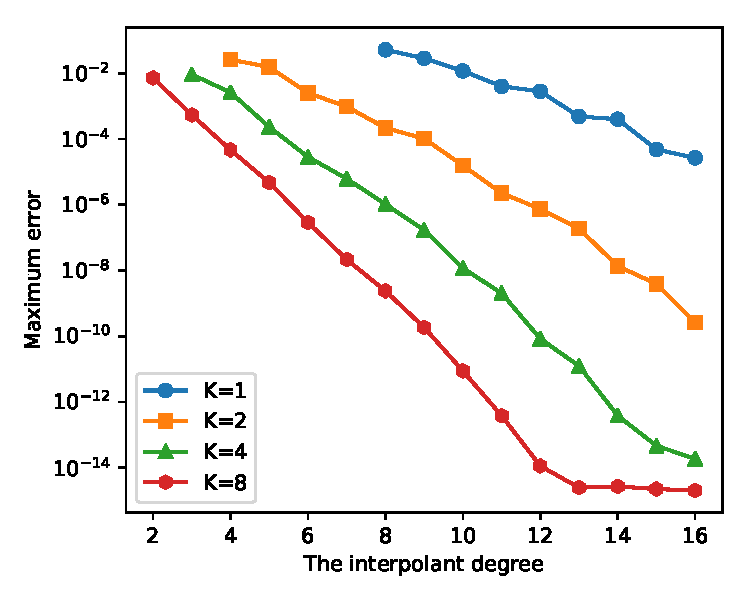
\includegraphics{tex/figures/interpolant_error}
	\fautor
	\label{fig:interpolant_error}
\end{figure}

\begin{figure}
	\centering
	\caption{The interpolation error measured on roots that were found after three Newton's iterations.}
	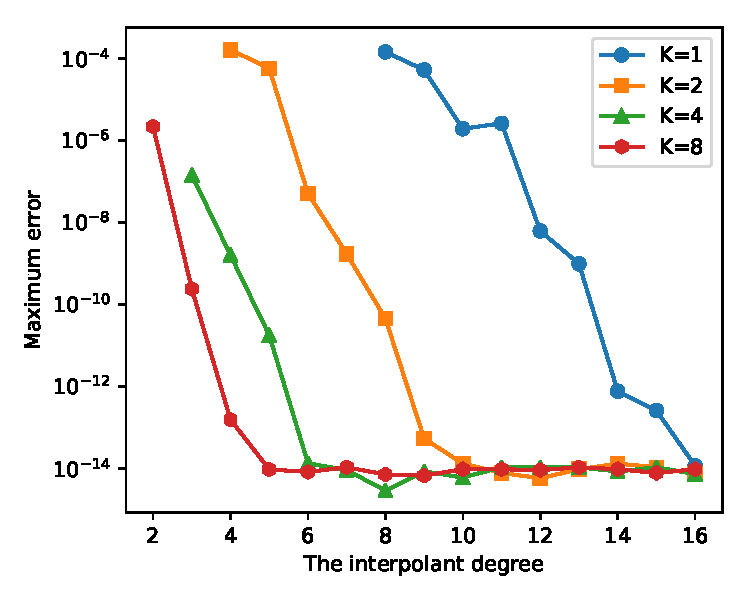
\includegraphics{tex/figures/interpolant_error_after_newton}
	\fautor
	\label{fig:interpolant_error_after_newton}
\end{figure}


\section{An Algorithm for MCER}\label{section:mcer}

This section introduces the elliptical PMCLP where there is no axis-parallel constraint, that is, the ellipses can be freely rotated. We refer to this problem as \sigla{MCER}{Maximal Covering by Ellipses with Rotation}. In comparison with MCE, this problem introduces a new a new variable which is responsible for determining the rotation angle of every ellipse making MCER a more challenging problem.

\section{Definition}

An instance of the non-axis-parallel is defined exactly like the axis-parallel one on \autoref{chapter:ellipses}. It is given by a set of demand points $\Pp=\{p_1, \dots, p_n\}$, $p_j\in\R^2$; a list of weights $\Ww:=\{w_1, \dots, w_n\}$, with $w_j\in\R_{\ge0}$ being the weight of point $p_j$;
and a set of $m$ axis-parallel ellipses given by their shape parameters $\Rr:=\{(a_1, b_1), \dots, (a_m, b_m)\}$, with $(a_j, b_j)\in\R_{>0}^2$ and $a_j>b_j$.
Additionally, to make the text more clear, we define a set of $m$ ellipses as $\E = \{E_1, \dots, E_m\}$, with $E_j : \R^2\times\R^2 \mapsto \R^2$ being a function that takes the center and angle of rotation where the $j$-th ellipse is located as input, and returns its coverage region.

Given an instance of $MCER$, we define $Q:=(q_1, \dots, q_m) \in \R^{2m}$ to be the centers of each ellipse, $\Theta:=(\theta_1, \dots, \theta_m) \in [0, \pi)^m$ to be the angle of rotation of each ellipse and $E_i(q_i, \theta_i)$ to be the coverage region of ellipse $E_i$ with its center at point $q_i$ rotated by angle $\theta_i$, which is given by \autoref{eq:rotated_ellipse_co}. Therefore MCER is defined as the problem of determining $Q$ and $\Theta$ (placing and rotating each ellipse) to maximize the weight of points covered by the $m$ ellipses, which is given by

\begin{equation}\label{eq:optMCEn}
\max_{Q, \Theta}{w\left(\bigcup_{i=1}^{m} \Pp \cap E_i(q_i, \theta_i)\right)}.
\end{equation}

An additional notation is used on this chapter, $\tilde{E_i}(q_i, \theta_i)$ is defined to be the set of points on the border of $E_i(q_i, \theta_i)$, specially, the operation $\Pp \cap \tilde{E_i}(q_i, \theta_i)$ is used to refer to the set of points from $\Pp$ that lie on the border of $E_i(q_i, \theta_i)$.


\begin{proposicao}\label{lema:mce_2b}
	Let $(\Pp, \E)$ be an instance of MCER. In an optimal solution of MCER, for any $E_j \in \E$, such that $|\Pp \cap E_j(q_j, \theta_j)|\ge2$, there is $q_j'$ such that $\Pp \cap E_j(q_j', \theta_j)=\Pp \cap E_j(q_j, \theta_j)$ and $\Pp \cap \tilde{E_j}(q_j', \theta_j) \ge 2$.
\end{proposicao}

\begin{demonstracao}
	First, the angle of rotation can be ignored as it does not change.
	
	Let $A=\Pp \cap E_j(q_j, \theta_j)$ be the set of points covered by $E_j$ and $X=\cap_{p \in A}E_j(p, \theta_j)$ be the region of intersection of ellipses centered at each point from $A$.

	As it was shown on \autoref{chapter:ellipses}, $X$ is a region that is limited by arcs of ellipses. As this region is the non-empty intersection of more than one ellipse, there are at least two of these arcs that encounter at one point creating a vertex. Selecting any of these vertices as $q_j'$ will make $|\Pp \cap \tilde{E}_j(q_j', \theta_j)| \ge 2$.
	
\end{demonstracao}

What \autoref{lema:mce_2b} is saying is that any optimal solution for MCER can be transformed into another optimal solution where every ellipse covers the same set of points and those which cover more than one point has two points on their border. Also, this equivalent optimal solution can be always achieved by just translating the ellipses. An example is shown on \autoref{fig:ellipse-2-points} for one ellipse.

A lot of the ideas developed in this chapter are based on fixing two points on the border of an ellipse, which is why \autoref{def:feasible_angle} introduces a new notation for angles that an ellipse rotated by it can be translated into a center, such that it contains two fixed points. 

\begin{figure}[H]
	\centering
	\caption{An optimal solution before and after applying \autoref{lema:mce_2b}.}
	\includegraphics{tex/figures/scripts/ellipse-2-points}
	\fautor
	\label{fig:ellipse-2-points}
\end{figure}

\begin{definicao}\label{def:feasible_angle}
	Let $E$ be an ellipse and $u, v \in \R^2$. An angle $\theta \in [0, \pi)$ is said to be $(E, u, v)$-feasible if there is $q \in \R^2$ such that $\{u, v\} \subset \tilde{E}(q, \theta)$.
\end{definicao}

On \autoref{fig:feasible-angle} two examples for \autoref{def:feasible_angle} are shown. On one of them, an ellipse is rotated by $\pi/4$ and it is located such that it contains the two fixed points on its border. That means $\pi/4$ is a $(E, u, v)$-feasible angle. On the other example, the ellipse is rotated by $\pi/2$ and there is not a center where the ellipse can be placed so it contains the two fixed points--they are too far apart. This makes $\pi/2$ a not $(E, u, v)$-feasible angle.

\begin{figure}
	\centering
	\caption{A $(E, u, v)$-feasible angle and a not $(E, u, v)$-feasible angle.}
	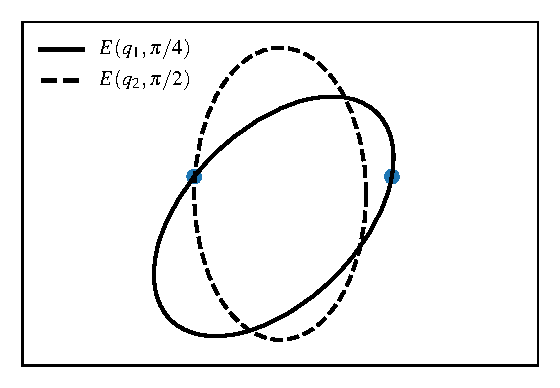
\includegraphics{tex/figures/scripts/feasible-angle}
	\fautor
	\label{fig:feasible-angle}
\end{figure}

\begin{lema}\label{lema:3pnts}
	Let $(\Pp, \E)$ be an instance of MCER, in an optimal solution, for any $E_j \in \E$, such that $|\Pp \cap E_j(q_j, \theta_j)|>2$, at least one of the two cases is true:
	
	\begin{enumerate}
		\item There is $q', \theta'$, and $\{u, v, w\} \subset \Pp \cap E_j(q_j, \theta_j)$, such that $\{u, v, w\} \subset \tilde{E}(q', \theta')$.
		
		\item Let $A=\Pp \cap E_j(q_j, \theta_j)$, and $u, v \in A$ such that there exists $\hat{q}_j$ such that $\{u, v\} \subset \tilde{E_j}(\hat{q}_j, \theta_j)$ and $A \subset E_j(\hat{q}_j, \theta_j)$. Then for any $(E_j, u, v)$-feasible angle $\theta \in [0, 2\pi]$, there exists $\bar{q}_j$ such that $\{u, v\} \subset \tilde{E_j}(\bar{q}_j, \theta)$ and $A \subset E_j(\bar{q}_j, \theta)$.
	\end{enumerate}
\end{lema}

The first case of \autoref{lema:3pnts} is saying that there is another optimal solution which has $E_j$ covering the same set of points, but with three points on its border. 

The second case of \autoref{lema:3pnts} says that after fixing a pair of points on the border of $E_j$ maintaining the covered set, for any angle that allows the two points to stay on the border of $E_j$, there is a center that maintains the covered set the same.

On \autoref{fig:lema-3-points} both cases of \autoref{lema:3pnts} are shown. There, it can be seen that for the second case, it does not matter which feasible angle by which the ellipse is rotated, the third point will always be inside the coverage area. Also, an example of the first case is shown where there are three points lie exactly on the border of the ellipse.

\begin{figure}
	\centering
	\caption{An example of \autoref{lema:3pnts}.}
	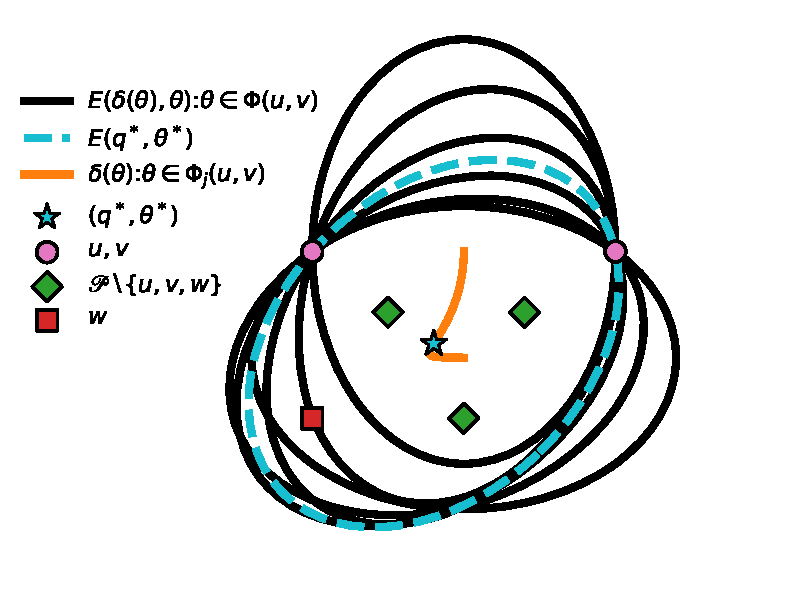
\includegraphics{tex/figures/scripts/lema-3-points}
	\fautor
	\label{fig:lema-3-points}
\end{figure}

The idea to prove \autoref{lema:3pnts} is that after fixing $u, v$ on the border of $E_j$, which is possible by \autoref{lema:mce_2b}, the movement of rotation and translation while keeping $u, v$ on the border is continuous. Because of that, the negation of case two implies case one and vice versa.


If we define an equivalence relation between optimal solutions as: $S_1$ is equivalent to $S_2$ if they both cover the same set of points, we can use \autoref{lema:3pnts} and \autoref{lema:mce_2b} to identify the equivalence classes. Let $S$ be any optimal solution, in $[S]$ (its equivalence class) there is another solution where any ellipse $E_j \in \E$ falls in at least one of the cases below:
\begin{itemize}
	\item $E_j$ covers only one point.
	\item $E_j$ covers more than one point with $u$ and $v$ being on the border of $E_j$. Note that there could be infinitely many of solutions like that, however, \autoref{lema:3pnts} guarantees that any $(E_j, u, v)$-feasible angle yields an equivalent optimal solution.
	\item $E_j$ covers more than two points with three of them on its border.
\end{itemize}

The following two sections will treat the second and third cases (the first case is trivial). Going through every possibility of an ellipse falling in any of the three cases guarantees that an optimal solution is found.

\section{Ellipse by two points}

Let $E$ be an ellipse with shape parameters $(a, b)\in \R^2_{>0}$ and $u, v\in \R^2$, one wants to find a $(E, u, v)$-feasible angle $\theta\in[0,\pi]$ and every center $q\in\R^2$ such that $\{u, v\} \subset \tilde{E}(q, \theta)$.

For a fixed angle, finding every center such that two points are on the border of the ellipse is done on \autoref{chapter:ellipses_intersection}, from there we know that there could be at most $2$ of such centers. The only thing left to be done is finding a feasible angle. It turns out that the angle that makes the major-axis of the ellipse to be aligned with the line that passes through $u$ and $v$ will be a feasible angle if, and only if the set of feasible angles is not empty. This can be seen geometrically as other angles achieve a lesser maximum distance between the two points on the border.

\section{Ellipse by three points}




\section{Improvements}\label{section:improvements}


In the CLS construction for MCER, calling the algorithm to determine every solution of E3P for every triplet of points can become expensive. To avoid that, given three points and an ellipse with shape parameters $(a, b)$, we can skip calling that  algorithm if the maximum distance between any of the points is greater than $2a$, or if the triangle's area with vertices on these three points have area greater than $\frac{3\sqrt{3}}{4}\pi ab$, which can be proved to be the greatest area of an inscribed triangle in an ellipse with shape parameters $(a, b)$.

%\section{Reducing the CLS size}\label{section:reducing_cls}
%As for the algorithms for both MCE and MCER, the number of solutions they go through is directly proportional to the size of each ellipse's CLS, reducing their size can significantly improve the performance of both algorithms. 

For MCE (the MCER's case is analogous), let $q, q' \in S_j$ be two possible locations in the CLS for the $j$-th ellipse. If $\Pp \cap E_j(q') \subset \Pp \cap E_j(q)$, then $q'$ is redundant and we can remove it from $S_j$, as it produces a solution which is either non-optimal or equivalent to an optimal one.

To remove redundant elements from a CLS, we use the same tree-like data structure described in \cite{andreta}, which keeps every maximal subset of covered points by an ellipse, and supports a query operation to verify if a subset is maximal or not.
First, we sort the elements in $S_j$ by the number of covered demand points, non-decreasingly. Then, we iterate over it, removing elements which make the ellipse cover non-maximal subsets of demand points, when compared to the elements of $S_j$ that have already been processed.


%\section{Prunning the Backtracking Tree}\label{section:prunning}
%In this section, we introduce a condition for skipping solutions in the backtracking process in the algorithms for MCE and MCER.
The idea is to prune the backtracking tree by observing that any solution constructed going down the current branch will have a value less than or equal to the current best solution.
As this condition can be applied for both problems, and their notation differs very little, we describe it only for MCE.

Given an instance $(\Pp, \Ww, \Rr)$ of MCE, an upper-bound for the value of an optimal solution is the sum of the optimal solutions for each ellipse individually:
\begin{equation}\label{eq:upper-1}
\max_{Q} w\left(\bigcup_{j=1}^m \Pp \cap E_j(q_j)\right) \le \sum_{j=1}^m \max_{q_j} w(\Pp \cap E_j(q_j)).
\end{equation}

Suppose that the first $k$ ellipses are fixed at locations $(q_1,\dots, q_k)$, and that we have a lower-bound $L$ for the value of an optimal solution. Let $Z_k=\Pp\setminus \cup_{j=1}^k E_j(q_j)$ be the points not covered by the first $k$ ellipses, then we can use \autoref{eq:upper-1} to verify if we can skip every solution where the first $k$ ellipses are fixed at  $(q_1,\dots, q_k)$ or not.
If
\begin{equation}\label{eq:upper}
w\left(\bigcup_{j=1}^{k} \Pp \cap E_j(q_j)\right)+
\sum_{j=k+1}^m \max_{q_j} w(Z_j \cap E_j(q_j)) \le L,
\end{equation}
then, any solution with the first $k$ ellipses fixed at $(q_1,\dots, q_k)$ will have value less than or equal to the value of an optimal solution, therefore, we can cut the backtracking tree there. In practice, we can use the value of the best solution found at the moment as the lower-bound $L$.

It is worth mentioning that this improvement do not have an effect in a possible worst case scenario. We decided to adopt it in our implementation because it showed good results in practice.
For example, without it, 
MCER-$k$'s algorithm takes nine seconds to obtain an optimal solution for instance AB060 developed by \cite{andreta}, going through \num{336494451} solutions, while the implementation using \autoref{eq:upper} to prune the backtracking tree for the same instance takes less than one second to return an optimal solution, and evaluates only \num{1809} solutions in total.


\section{Implementation Details}\label{section:implementation}
In this section, we give more details about the implementation of the algorithms developed in our work.

All the algorithms were implemented using the C++ language, compiled with g++ (G++ 6.3.0) with the optimization flag -O3. The actual code is available in \url{https://sites.icmc.usp.br/andretta/tedeschi-2020/}.

\subsection{Determining the eigenvalues of a matrix}

In the algorithm to obtain every solution of E3P described in \autoref{section:e3p}, we assumed that a procedure which returns every eigenvalue of a given complex matrix was available. In practice, we used the famous linear algebra package LAPACK (see \cite{lapack} for more details).
Even though LAPACK is a library for the FORTRAN programming language, its routines can be made available in a C/C++ environment by simply adding the \textit{-llapack} linking flag to the compilation. The only remarks, though, are that FORTRAN represents matrices in a column-major fashion, and receives parameters only by reference. Therefore, matrices must be transposed before being passed to a routine, and every parameter must receive a pointer to a variable containing its value.

To compute every eigenvalue of a complex matrix, LAPACK offers a routine called ZGEEV, which is an implementation of the QR algorithm.
This routine optionally can also be asked to compute the right or left eigenvectors depending on two of its parameters. 

% ZGEEV receives in total $14$ parameters, with $4$ of them being used for output. 

\subsection{Symbolic computation}


Back in \autoref{section:e3p}, we were faced with the problem of writing function $\xi$ defined in \autoref{eq:xi} as a complex polynomial in the new variable $z=e^{i\theta}$. We suggested that symbolic computation should be used for this task, as the expressions for that polynomial's coefficients become very long, and doing that by hand is, to say the least, a very tedious work.
Symbolic computation is a vast topic, which deals with the problem of solving or manipulating mathematical expressions computationally. 
In practice, we utilized an external library for Python called SymPy (see \cite{sympy} for more information).
This tool can create expressions using arithmetic operators on predefined symbols, numbers, and other expressions. It can also convert expressions into polynomials in the power format, and output them directly into C code. Using these features, we wrote $\xi(\theta)(e^{i\theta})^6$ as a polynomial by replacing the sine and cosine functions by the identities $\cos\theta=(z+z^{-1})/2$ and $\sin\theta=(z+z^{-1})/(2i)$.

%The actual coefficients of that polynomial would take more than ten pages if they were to be presented here, because of that, we made them available elsewhere in \url{https://sites.icmc.usp.br/andretta/tedeschi-2020/}.

\section{Numerical Experiments}\label{section:numerical}
The goal of this chapter is to show in practice the results of the algorithms for MCE and MCER proposed by us. We first give some implementation details, then we start discuss the solutions obtained for instances proposed in past works, and finally we propose some new instances with the intention of finding the limits of our algorithms.

\section{Implementation}

All the algorithms were implemented using the C++ language, with compiler g++ (G++ 6.3.0). To activate the optimization of compilation we used the -O4 flag.. All the experiments were run in a computer with the following specification:
\begin{itemize}
	\item CPU Intel(R) Core(TM) i7-2600 CPU @ 3.40GHz;
	\item 16Gib of RAM memory;
	\item Linux Operating System: Debian 4.19.5.
\end{itemize}
\subsection{Determining the eigenvalues of a matrix}

In \autoref{algoritmo:e3p}, we assumed that a procedure which returns every eigenvalue of a given square matrix was available. In practice, we used the very famous linear algebra package LAPACK (see \citeonline{lapack} for more details).
LAPACK is a library for the FORTRAN programming language. However, its routines can be made available in a C/C++ environment by simply adding the -llapack linking flag to the compilation. The only remarks, though, are that FORTAN represents matrices in a column-major fashion, and receives parameters only by reference. Therefore, matrices must be transposed before being passed to a routine, and every parameter must receive a pointer to a variable containing its value.

LAPACK offers a routine called ZGEEV that computes every eigenvalue of a complex matrix by using an implementation of the QR algorithm. 
This routine optionally can also be asked to compute the right or left eigenvectors depending on two of its parameters. 
ZGEEV receives in total $14$ parameters, with $4$ of them being used for output. We show a brief description of them in \autoref{tab:zgeev} along with the specification of the value we set each parameter in our implementation.
%\renewcommand{\arraystretch}{1.1}

\begin{table}[H]\label{tab:zgeev}
	\begin{center}
	\begin{tabular}{|c|m{18em}|m{8em}|}
		
		\hline
		\textbf{Parameter} & \multicolumn{1}{c|}{\textbf{Description}} & \multicolumn{1}{c|}{\textbf{Value}}\\
		\hline
		JOBVL&  Indicates whether to compute the left eigenvalues&  'N' (no eigenvectors should be computed)\\
		\hline
		JOBVR&  Indicates whether to compute the right eigenvalues&  'N' (no eigenvectors should be computed)\\
		\hline
		N    &  Order of matrix A &  6\\
		\hline
		A    &  The square matrix whose eigenvalues are to be computed & The companion matrix \\
		\hline
		LDA  &  Leading dimension of A & 6 \\
		\hline
		W    &  The eigenvalues output array &  A complex array of size 6\\
		\hline
		VL   &  The left eigenvectors output array & A complex array of size 1 \\
		\hline
		LDVL &  Leading dimension of VL&  1\\
		\hline
		VR   &  The right eigenvectors output array&  A complex array of size 1\\
		\hline
		LDVR &  Leading dimension of VR&  1\\
		\hline
		WORK &  A workspace for the procedure to utilize&  A complex array of size 12\\
		\hline
		LWORK&  Dimension of WORK &  12\\
		\hline
		RWORK&  A real workspace of size 2N &  A double array of size 12\\
		\hline
		INFO &  An integer containing $0$ if the algorithm was able to compute every eigenvalue &  A pointer to an integer variable\\
		\hline
	\end{tabular}
	\end{center}
	\caption{The ZGEEV's parameter list.}
\end{table}

\subsection{Symbolic Computation}

Symbolic computation is a vast topic, which deals with the problem of solving or manipulating mathematical expressions computationally. 

Back in \autoref{chapter:e3p}, we were faced with the problem of writing the function $\xi$ defined in \autoref{eq:circumscribed_circle_b} as a complex polynomial in the power format by replacing the sine and cosine functions with the identities given by  \autoref{eq:complex_trig_cos} and \autoref{eq:complex_trig_sin}.

As expected, computing the coefficients of that polynomial in terms of the E3P's instance by hand is very challenging; the expressions get too long, and it becomes humanly impossible not to make any mistake. 
For that reason, we resort to Symbolic computation for this task.

In practice, we utilized an external library for Python called SymPy (see \citeonline{sympy} for more information).
This tool can create expressions using arithmetic operators on predefined symbols, numbers, and other expressions. It can also convert expressions into polynomials in the power format, and output them directly into C code. Using these features, we can write $\xi(\theta)(e^{i\theta})^6$ as a polynomial by replacing the sine and cosine functions with expressions for the identities given by  \autoref{eq:complex_trig_cos} and \autoref{eq:complex_trig_sin}, and then import it into our C++ implementation of \autoref{algoritmo:e3p} by printing the polynomial's list of coefficients as C code.

%This can be done by creating a composition of an expression for $\xi(\theta)(e^{i\theta})^6$ with the expressions for $\cos(\theta)$ and $\sin(\theta)$ defined by \autoref{eq:complex_trig_cos} and \autoref{eq:complex_trig_sin}.
%After that, running a command, we can ask SymPy to transform that expression into a polynomial informing it that its variable is $z=e^{i\theta}$. Finally, very conveniently for us, SymPy has a function that outputs expressions directly as C code, which can be used to import the polynomial into our implementation of \autoref{algoritmo:e3p}.

\subsection{Some details and improvements}\label{section:improvements}

To achieve the results that are shown later in this chapter, an efficient implementation of \autoref{algoritmo:mce} and \autoref{algoritmo:mcer} had to be done. Just translating those algorithms into a programming language was not enough to obtain solutions for every instance previously published in \citeonline{andreta}.
Therefore, we present here, some improvements that can be applied to the implementation of those algorithms, which can result in a significant improvement in performance, especially in terms of CPU time.

In both algorithms, a subroutine to construct an ellipse's CLS is called inside the backtracking routine. This can potentially make the same combination of points be considered multiple times.
To avoid this unnecessary computation, points that have already been considered for an ellipse's CLS can be stored, and only new combinations can then be taken into account each time the CLS subroutine is called. 

Another improvement that can be made in the construction of an ellipse's CLS is the elimination of redundant solutions.
Let $(Q, \Theta)$ and $(Q', \Theta')$ be two solutions of MCER. If, for any $j \in \{1, \dots, m\}$, we have $\Pp \cap E_j(q_j', \theta_j') \subset \Pp \cap E(q_j, \theta_j)$, then we can for sure dismiss solution $(Q', \Theta')$.
In our implementation, we use the same tree-like data structure as the one described by \citeonline{andreta} to only keep solutions that are not redundant.

Also, to avoid solving the subproblem E3P in the algorithm for MCER, we can check if the maximum distance between any of the three points is greater than $2a$, where $a$ is an ellipse's semi-major. This is useful because calling \autoref{algoritmo:e3p} for every triplet of points of an instance of MCER can be very expensive.

The last implementation improvement was obtained by keeping an upper-bound, which can be used to skip solutions that are surely not better than the current best solution.
When the backtracking algorithm has the location for the first $j$ ellipses fixed, we want to have an upper-bound for the best solution that can still be found by choosing the location of the $m-j$ remaining ellipses.
Let us consider the case for the MCER's algorithm (the MCE's case is analogous). Let $$z_j = \max_{(q, \theta) \in S_j} w(\Pp \cap E_j(q, \theta)),$$ and $OPT_j$ be the value of the best solution which has the first $j$ ellipses fixed at $(q_1, \theta_1); \dots; (q_j, \theta_j)$. Then, as $z_k$ is the best value that the $k$-th ellipse can contribute to any solution, we get the following inequality
\begin{equation*}
OPT_j \le w\left(\bigcup_{k=1}^{j} \Pp \cap E_k(q_k, \theta_k)\right) + \sum_{k=j+1}^m z_k.
\end{equation*}
This upper-bound is easy to compute as $\{z_1, \dots, z_m\}$ can be preprocessed, and the weight of every point covered so far in the backtrack can be obtained by adding another parameter to the $MCER_{bt}$ procedure.
Let $OPT$ be the current optimal solution, we have that if
\begin{equation}
\label{eq:upper-bound}
w\left(\bigcup_{k=1}^{j} \Pp \cap E_k(q_k, \theta_k)\right) + \sum_{k=j+1}^m z_k \le OPT,
\end{equation}
then $OPT_j \le OPT$, which means that we can skip every solution with the first $j$ ellipses fixed at $(q_1, \theta_1); \dots; (q_j, \theta_j)$.

It is worth pointing out that these improvement suggestions do not have an effect in a possible worst case scenario. We are adopting them in our implementation because they showed good results in practice.
For example, without taking the suggestion given by \autoref{eq:upper-bound}, \autoref{algoritmo:mcer-k} takes nine seconds to obtain an optimal solution for instance AB060, going through \num{336494451} solutions.
In \autoref{tab:mcer-results-ab1}, we show the results of \autoref{algoritmo:mcer-k} implemented with all the improvement suggestions given here; for the instance AB060, the algorithm takes less than one second to return an optimal solution, and evaluates only \num{1809} solutions.

\section{A greedy algorithm}

In \citeonline{church:1974} a simple greedy algorithm was introduced to compare the results obtained by the other algorithms developed by them. We do the same here and define a general greedy algorithm, which follows the same approach as the one in \citeonline{church:1974}, that works for both MCE and MCER.

Let $(\Pp, \Ww, \Rr)$ be an instance of MCE or MCER. Then, at the $j$-th iteration of the algorithm we choose the solution for the first ellipse. Considering $Z_j \subset \Pp$ as the set of uncovered points before the $j$-th iteration. Then, we set the solution for the $j$-th ellipse, as the solution of an instance of MCE-1 or MCER-1 with demand points $Z_j$.
That is the same as choosing, among all the possibilities in the $j$-th ellipse's CLS, the solution which maximizes the weight of covered points in $Z_j$.

\section{Results for known instances}

In this section, we present the results of \autoref{algoritmo:mce-k} and \autoref{algoritmo:mcer-k} for the instances CM1,CM2, CM4, CM5, CM7, CM8 proposed by \citeonline{canbolat}, and for the instances CM3,CM6,CM9 and AB001-AB120 proposed by \citeonline{andreta}.

For each instance, we display the selected ellipses and the income of the found optimal solution. 
We also display some performance metrics with the intention of giving an idea of how much computation had to be done for the algorithms to find an optimal solution. These metrics are: 
the CLS size of every ellipse, the number of nodes in the backtracking tree, the number of leaves corresponding to a solution in the backtracking tree, the CPU time spent on constructing the CLSs, and the total CPU time.
For the algorithms for MCER, we also have a column for the number of E3P subproblems that were solved, not counting the triplet of points which are dismissed by the improvements suggestions given in \autoref{section:improvements}.


\subsection{MCE-$k$}

In \autoref{tab:mce-results-cm}, the results for instances CM1-CM9 are shown. 
The algorithm proposed here showed great results as it was able to obtain optimal solutions in less than one second for every one of the instances CM1-CM9.
Even though the experiments were run in a different environment, we can still say that this is a great improvement compared with the results from \citeonline{andreta}. For example, to obtain an optimal solution for the instance CM9, the method proposed by \citeonline{andreta} took more than thirty minutes.
In \autoref{tab:mce-results-ab1} and \autoref{tab:mce-results-ab2}, we present the results for instances AB001-AB120. The only instance that our algorithm took more than one second to return an optimal solution was AB120, which it took 1.08 second.

In practice, at least for these instances, the bound $\bigO(n^{3m})$ for the algorithm for MCE-$k$ seems to be loose. In instance CM9, for example, this bound says that the number of leaves corresponding to a solution in the backtracking tree should be close to $n^{3m} = (10^2)^{3\times 3} = 10^{18}$, which is very far from the actual number of $649$ such leaves obtained in practice.
This is also the case for the size of the CLSs, which are all very far away from its $\bigO(n^2)$ bound. The greatest CLS size observed was $174$ for instance CM9, which is still very far away from $n^2$, which in this case is $10^4$.
\begin{table}
	\begin{center}
		\resizebox{\textwidth}{!}{%
			
			\begin{tabular}{|cccc|cr|crrrr|}
				\hline
				\multicolumn{4}{|c|}{Instance} & \multicolumn{2}{c|}{Optimal Solution} & \multicolumn{5}{c|}{Performance metrics}\\
				\hline
				
				%%% Second line of header
				
				\multirow{2}{*}{Name} & 
				\multirow{2}{*}{$n$} & 
				\multirow{2}{*}{$m$} & 
				\multirow{2}{*}{$k$} & 
				Selected & 
				\multirow{2}{*}{Income} & 
				CLS size&
				\multicolumn{2}{c}{Backtracking Tree} & 
				\multicolumn{2}{c|}{\centering CPU Time (s)}\\
				& & & & \centering Ellipses & & $|S_k|$ & \# nodes & \# sol. leaves & CLS-MCE & Total\\
				\hline
				CM1&\multirow{3}{*}{\num{25}}&\multirow{3}{*}{\num{3}}&\num{1}&\num{1}\num{2},\num{3},&\num{3.0}&\num{19}&\num{58}&\num{18}&\num{0.00}&\num{0.00}
\\CM2& & &\num{2}&\num{1},\num{2}\num{3},&\num{3.0}&\num{21}&\num{58}&\num{18}&\num{0.00}&\num{0.00}
\\CM3& & &\num{3}&\num{1},\num{2},\num{3}&\num{3.0}&\num{19}&\num{58}&\num{18}&\num{0.00}&\num{0.00}
\\\hline
CM4&\multirow{3}{*}{\num{50}}&\multirow{3}{*}{\num{3}}&\num{1}&\num{1}\num{2},\num{3},&\num{10.0}&\num{43}&\num{141}&\num{50}&\num{0.00}&\num{0.00}
\\CM5& & &\num{2}&\num{1},\num{2}\num{3},&\num{10.0}&\num{47}&\num{141}&\num{50}&\num{0.00}&\num{0.00}
\\CM6& & &\num{3}&\num{1},\num{2},\num{3}&\num{10.0}&\num{50}&\num{141}&\num{50}&\num{0.00}&\num{0.00}
\\\hline
CM7&\multirow{3}{*}{\num{100}}&\multirow{3}{*}{\num{3}}&\num{1}&\num{1}\num{2},\num{3},&\num{25.0}&\num{101}&\num{924}&\num{687}&\num{0.02}&\num{0.02}
\\CM8& & &\num{2}&\num{1},\num{2}\num{3},&\num{25.0}&\num{135}&\num{924}&\num{687}&\num{0.02}&\num{0.02}
\\CM9& & &\num{3}&\num{1},\num{2},\num{3}&\num{25.0}&\num{174}&\num{924}&\num{687}&\num{0.02}&\num{0.02}
\\
				\hline
				
			\end{tabular}
		}
		\caption{Solutions of MCE-$k$ for instances CM1-CM9.}
		\label{tab:mce-results-cm}
	\end{center}
\end{table}

\begin{table}
	\begin{center}
		\resizebox{0.85\textwidth}{!}{%
			
			\begin{tabular}{|cccc|cr|crrrr|}
				\hline
				\multicolumn{4}{|c|}{Instance} & \multicolumn{2}{c|}{Optimal Solution} & \multicolumn{5}{c|}{Performance metrics}\\
				\hline
				
				%%% Second line of header
				
			\multirow{2}{*}{Name} & 
			\multirow{2}{*}{$n$} & 
			\multirow{2}{*}{$m$} & 
			\multirow{2}{*}{$k$} & 
			Selected & 
			\multirow{2}{*}{Income} & 
			CLS size&
			\multicolumn{2}{c}{Backtracking Tree} & 
			\multicolumn{2}{c|}{\centering CPU Time (s)}\\
			& & & & \centering Ellipses & & $|S_k|$ & \# nodes & \# sol. leaves & CLS-MCE & Total\\
				\hline
				AB001&\multirow{0}{*}{\num{10}}&\multirow{0}{*}{\num{3}}&\num{1}&\num{2}&\num{1.4}&\multirow{0}{*}{\num{10}}&\num{32}&\num{11}&\num{0.00}&\num{0.00}
\\AB002& & &\num{2}&\num{2},\num{3}&\num{2.3}& &\num{66}&\num{8}&\num{0.00}&\num{0.00}
\\AB003& & &\num{3}&\num{1},\num{2},\num{3}&\num{2.8}& &\num{162}&\num{6}&\num{0.00}&\num{0.00}
\\\hline
AB004&\multirow{3}{*}{\num{10}}&\multirow{3}{*}{\num{4}}&\num{1}&\num{4}&\num{0.9}&\multirow{3}{*}{\num{10}}&\num{41}&\num{10}&\num{0.00}&\num{0.00}
\\AB005& & &\num{2}&\num{2},\num{4}&\num{1.4}& &\num{159}&\num{98}&\num{0.00}&\num{0.00}
\\AB006& & &\num{3}&\num{2},\num{3},\num{4}&\num{1.8}& &\num{312}&\num{112}&\num{0.00}&\num{0.00}
\\AB007& & &\num{4}&\num{1},\num{2},\num{3},\num{4}&\num{1.0}& &\num{1150}&\num{60}&\num{0.00}&\num{0.00}
\\\hline
AB008&\multirow{4}{*}{\num{10}}&\multirow{4}{*}{\num{5}}&\num{1}&\num{5}&\num{0.9}&\multirow{4}{*}{\num{10}}&\num{54}&\num{10}&\num{0.00}&\num{0.00}
\\AB009& & &\num{2}&\num{3},\num{5}&\num{1.4}& &\num{172}&\num{98}&\num{0.00}&\num{0.00}
\\AB010& & &\num{3}&\num{3},\num{4},\num{5}&\num{1.8}& &\num{286}&\num{56}&\num{0.00}&\num{0.00}
\\AB011& & &\num{4}&\num{2},\num{3},\num{4},\num{5}&\num{1.0}& &\num{1492}&\num{120}&\num{0.00}&\num{0.00}
\\AB012& & &\num{5}&\num{1},\num{2},\num{3},\num{4},\num{5}&\num{-1.5}& &\num{8693}&\num{7}&\num{0.00}&\num{0.00}
\\\hline
AB013&\multirow{5}{*}{\num{20}}&\multirow{5}{*}{\num{3}}&\num{1}&\num{2}&\num{1.4}&\multirow{5}{*}{\num{20}}&\num{58}&\num{21}&\num{0.00}&\num{0.00}
\\AB014& & &\num{2}&\num{2},\num{3}&\num{2.3}& &\num{198}&\num{18}&\num{0.00}&\num{0.00}
\\AB015& & &\num{3}&\num{1},\num{2},\num{3}&\num{2.8}& &\num{573}&\num{16}&\num{0.00}&\num{0.00}
\\\hline
AB016&\multirow{3}{*}{\num{20}}&\multirow{3}{*}{\num{4}}&\num{1}&\num{2}&\num{1.5}&\multirow{3}{*}{\num{20}}&\num{73}&\num{22}&\num{0.00}&\num{0.00}
\\AB017& & &\num{2}&\num{2},\num{3}&\num{2.9}& &\num{192}&\num{36}&\num{0.00}&\num{0.00}
\\AB018& & &\num{3}&\num{2},\num{3},\num{4}&\num{3.8}& &\num{645}&\num{15}&\num{0.00}&\num{0.00}
\\AB019& & &\num{4}&\num{1},\num{2},\num{3},\num{4}&\num{4.0}& &\num{6331}&\num{37}&\num{0.00}&\num{0.00}
\\\hline
AB020&\multirow{4}{*}{\num{20}}&\multirow{4}{*}{\num{5}}&\num{1}&\num{4}&\num{2.4}&\multirow{4}{*}{\num{20}}&\num{82}&\num{21}&\num{0.00}&\num{0.00}
\\AB021& & &\num{2}&\num{3},\num{4}&\num{3.9}& &\num{131}&\num{18}&\num{0.00}&\num{0.00}
\\AB022& & &\num{3}&\num{3},\num{4},\num{5}&\num{4.8}& &\num{569}&\num{29}&\num{0.00}&\num{0.00}
\\AB023& & &\num{4}&\num{2},\num{3},\num{4},\num{5}&\num{4.0}& &\num{8681}&\num{108}&\num{0.00}&\num{0.00}
\\AB024& & &\num{5}&\num{1},\num{2},\num{3},\num{4},\num{5}&\num{2.5}& &\num{54810}&\num{229}&\num{0.00}&\num{0.00}
\\\hline
AB025&\multirow{5}{*}{\num{30}}&\multirow{5}{*}{\num{3}}&\num{1}&\num{1}&\num{2.5}&\multirow{5}{*}{\num{27}}&\num{74}&\num{29}&\num{0.00}&\num{0.00}
\\AB026& & &\num{2}&\num{1},\num{2}&\num{4.9}& &\num{166}&\num{50}&\num{0.00}&\num{0.00}
\\AB027& & &\num{3}&\num{1},\num{2},\num{3}&\num{6.8}& &\num{769}&\num{22}&\num{0.00}&\num{0.00}
\\\hline
AB028&\multirow{3}{*}{\num{30}}&\multirow{3}{*}{\num{4}}&\num{1}&\num{2}&\num{2.5}&\multirow{3}{*}{\num{28}}&\num{101}&\num{30}&\num{0.00}&\num{0.00}
\\AB029& & &\num{2}&\num{2},\num{3}&\num{4.9}& &\num{420}&\num{52}&\num{0.00}&\num{0.00}
\\AB030& & &\num{3}&\num{1},\num{2},\num{3}&\num{6.1}& &\num{1933}&\num{109}&\num{0.00}&\num{0.00}
\\AB031& & &\num{4}&\num{1},\num{2},\num{3},\num{4}&\num{7.0}& &\num{16219}&\num{456}&\num{0.00}&\num{0.00}
\\\hline
AB032&\multirow{4}{*}{\num{30}}&\multirow{4}{*}{\num{5}}&\num{1}&\num{3}&\num{2.5}&\multirow{4}{*}{\num{27}}&\num{119}&\num{29}&\num{0.00}&\num{0.00}
\\AB033& & &\num{2}&\num{3},\num{4}&\num{4.9}& &\num{472}&\num{49}&\num{0.00}&\num{0.00}
\\AB034& & &\num{3}&\num{2},\num{3},\num{4}&\num{7.1}& &\num{1621}&\num{22}&\num{0.00}&\num{0.00}
\\AB035& & &\num{4}&\num{2},\num{3},\num{4},\num{5}&\num{9.0}& &\num{12208}&\num{17}&\num{0.00}&\num{0.00}
\\AB036& & &\num{5}&\num{1},\num{2},\num{3},\num{4},\num{5}&\num{9.5}& &\num{179281}&\num{53}&\num{0.00}&\num{0.01}
\\\hline
AB037&\multirow{5}{*}{\num{40}}&\multirow{5}{*}{\num{3}}&\num{1}&\num{1}&\num{2.5}&\multirow{5}{*}{\num{37}}&\num{102}&\num{39}&\num{0.00}&\num{0.00}
\\AB038& & &\num{2}&\num{1},\num{2}&\num{4.9}& &\num{315}&\num{70}&\num{0.00}&\num{0.00}
\\AB039& & &\num{3}&\num{1},\num{2},\num{3}&\num{6.8}& &\num{1441}&\num{65}&\num{0.00}&\num{0.00}
\\\hline
AB040&\multirow{3}{*}{\num{40}}&\multirow{3}{*}{\num{4}}&\num{1}&\num{1}&\num{5.2}&\multirow{3}{*}{\num{37}}&\num{125}&\num{40}&\num{0.00}&\num{0.00}
\\AB041& & &\num{2}&\num{1},\num{4}&\num{7.1}& &\num{393}&\num{97}&\num{0.00}&\num{0.00}
\\AB042& & &\num{3}&\num{1},\num{2},\num{4}&\num{8.6}& &\num{2904}&\num{116}&\num{0.00}&\num{0.00}
\\AB043& & &\num{4}&\num{1},\num{2},\num{3},\num{4}&\num{10.0}& &\num{28554}&\num{296}&\num{0.00}&\num{0.00}
\\\hline
AB044&\multirow{4}{*}{\num{40}}&\multirow{4}{*}{\num{5}}&\num{1}&\num{3}&\num{3.5}&\multirow{4}{*}{\num{36}}&\num{148}&\num{38}&\num{0.00}&\num{0.00}
\\AB045& & &\num{2}&\num{1},\num{3}&\num{7.0}& &\num{754}&\num{68}&\num{0.00}&\num{0.00}
\\AB046& & &\num{3}&\num{1},\num{2},\num{3}&\num{9.2}& &\num{3847}&\num{61}&\num{0.00}&\num{0.00}
\\AB047& & &\num{4}&\num{1},\num{2},\num{3},\num{5}&\num{11.1}& &\num{33846}&\num{99}&\num{0.00}&\num{0.00}
\\AB048& & &\num{5}&\num{1},\num{2},\num{3},\num{4},\num{5}&\num{12.5}& &\num{524078}&\num{60}&\num{0.00}&\num{0.01}
\\\hline
AB049&\multirow{5}{*}{\num{50}}&\multirow{5}{*}{\num{3}}&\num{1}&\num{1}&\num{5.5}&\multirow{5}{*}{\num{42}}&\num{120}&\num{44}&\num{0.00}&\num{0.00}
\\AB050& & &\num{2}&\num{1},\num{2}&\num{7.9}& &\num{605}&\num{278}&\num{0.00}&\num{0.00}
\\AB051& & &\num{3}&\num{1},\num{2},\num{3}&\num{9.8}& &\num{2429}&\num{436}&\num{0.00}&\num{0.00}
\\\hline
AB052&\multirow{3}{*}{\num{50}}&\multirow{3}{*}{\num{4}}&\num{1}&\num{1}&\num{5.2}&\multirow{3}{*}{\num{46}}&\num{161}&\num{49}&\num{0.00}&\num{0.00}
\\AB053& & &\num{2}&\num{1},\num{2}&\num{8.7}& &\num{590}&\num{130}&\num{0.00}&\num{0.00}
\\AB054& & &\num{3}&\num{1},\num{2},\num{3}&\num{11.1}& &\num{3420}&\num{512}&\num{0.00}&\num{0.00}
\\AB055& & &\num{4}&\num{1},\num{2},\num{3},\num{4}&\num{13.0}& &\num{48977}&\num{1181}&\num{0.00}&\num{0.00}
\\\hline
AB056&\multirow{4}{*}{\num{50}}&\multirow{4}{*}{\num{5}}&\num{1}&\num{1}&\num{3.5}&\multirow{4}{*}{\num{44}}&\num{209}&\num{46}&\num{0.00}&\num{0.00}
\\AB057& & &\num{2}&\num{1},\num{4}&\num{6.9}& &\num{1650}&\num{126}&\num{0.00}&\num{0.00}
\\AB058& & &\num{3}&\num{1},\num{3},\num{4}&\num{9.4}& &\num{8061}&\num{656}&\num{0.00}&\num{0.01}
\\AB059& & &\num{4}&\num{1},\num{2},\num{3},\num{4}&\num{11.6}& &\num{71184}&\num{2016}&\num{0.00}&\num{0.01}
\\AB060& & &\num{5}&\num{1},\num{2},\num{3},\num{4},\num{5}&\num{13.5}& &\num{1971099}&\num{649}&\num{0.00}&\num{0.05}
\\
				\hline
				
			\end{tabular}
		}
		\caption{Solutions of MCE-$k$ for instances AB001-AB060.}
		\label{tab:mce-results-ab1}
	\end{center}
\end{table}

\begin{table}
	\begin{center}
		\resizebox{0.85\textwidth}{!}{%
			
			\begin{tabular}{|cccc|cr|crrrr|}
				\hline
				\multicolumn{4}{|c|}{Instance} & \multicolumn{2}{c|}{Optimal Solution} & \multicolumn{5}{c|}{Performance metrics}\\
				\hline
				
				%%% Second line of header
\multirow{2}{*}{Name} & 
\multirow{2}{*}{$n$} & 
\multirow{2}{*}{$m$} & 
\multirow{2}{*}{$k$} & 
Selected & 
\multirow{2}{*}{Income} & 
CLS size&
\multicolumn{2}{c}{Backtracking Tree} & 
\multicolumn{2}{c|}{\centering CPU Time (s)}\\
& & & & \centering Ellipses & & $|S_k|$ & \# nodes & \#sol. leaves & CLS-MCE & Total\\
				\hline
				AB061&\multirow{3}{*}{\num{60}}&\multirow{3}{*}{\num{3}}&\num{1}&\num{1}&\num{3.5}&\num{38}&\num{140}&\num{56}&\num{0.00}&\num{0.00}
\\AB062& & &\num{2}&\num{1},\num{2}&\num{5.9}&\num{41}&\num{440}&\num{103}&\num{0.00}&\num{0.00}
\\AB063& & &\num{3}&\num{1},\num{2},\num{3}&\num{7.8}&\num{54}&\num{2622}&\num{48}&\num{0.00}&\num{0.00}
\\\hline
AB064&\multirow{4}{*}{\num{60}}&\multirow{4}{*}{\num{4}}&\num{1}&\num{1}&\num{5.2}&\num{51}&\num{196}&\num{54}&\num{0.00}&\num{0.00}
\\AB065& & &\num{2}&\num{1},\num{2}&\num{8.7}&\num{44}&\num{1044}&\num{98}&\num{0.00}&\num{0.00}
\\AB066& & &\num{3}&\num{1},\num{2},\num{3}&\num{12.1}&\num{39}&\num{4275}&\num{130}&\num{0.00}&\num{0.00}
\\AB067& & &\num{4}&\num{1},\num{2},\num{3},\num{4}&\num{14.0}&\num{51}&\num{90366}&\num{77}&\num{0.00}&\num{0.01}
\\\hline
AB068&\multirow{5}{*}{\num{60}}&\multirow{5}{*}{\num{5}}&\num{1}&\num{3}&\num{4.5}&\num{62}&\num{267}&\num{54}&\num{0.01}&\num{0.01}
\\AB069& & &\num{2}&\num{1},\num{3}&\num{9.0}&\num{59}&\num{3479}&\num{102}&\num{0.01}&\num{0.01}
\\AB070& & &\num{3}&\num{1},\num{3},\num{4}&\num{12.4}&\num{42}&\num{25920}&\num{663}&\num{0.00}&\num{0.01}
\\AB071& & &\num{4}&\num{1},\num{2},\num{3},\num{4}&\num{14.6}&\num{43}&\num{198004}&\num{1603}&\num{0.01}&\num{0.01}
\\AB072& & &\num{5}&\num{1},\num{2},\num{3},\num{4},\num{5}&\num{16.5}&\num{52}&\num{5075488}&\num{1089}&\num{0.01}&\num{0.11}
\\\hline
AB073&\multirow{3}{*}{\num{70}}&\multirow{3}{*}{\num{3}}&\num{1}&\num{1}&\num{4.5}&\num{54}&\num{168}&\num{61}&\num{0.00}&\num{0.00}
\\AB074& & &\num{2}&\num{1},\num{2}&\num{7.9}&\num{48}&\num{370}&\num{111}&\num{0.00}&\num{0.00}
\\AB075& & &\num{3}&\num{1},\num{2},\num{3}&\num{9.8}&\num{59}&\num{3725}&\num{51}&\num{0.00}&\num{0.00}
\\\hline
AB076&\multirow{4}{*}{\num{70}}&\multirow{4}{*}{\num{4}}&\num{1}&\num{1}&\num{5.2}&\num{55}&\num{212}&\num{63}&\num{0.00}&\num{0.00}
\\AB077& & &\num{2}&\num{1},\num{2}&\num{9.7}&\num{43}&\num{696}&\num{114}&\num{0.01}&\num{0.01}
\\AB078& & &\num{3}&\num{1},\num{2},\num{3}&\num{13.1}&\num{43}&\num{5080}&\num{102}&\num{0.00}&\num{0.00}
\\AB079& & &\num{4}&\num{1},\num{2},\num{3},\num{4}&\num{16.0}&\num{60}&\num{113819}&\num{46}&\num{0.00}&\num{0.01}
\\\hline
AB080&\multirow{5}{*}{\num{70}}&\multirow{5}{*}{\num{5}}&\num{1}&\num{1}&\num{5.5}&\num{68}&\num{282}&\num{59}&\num{0.01}&\num{0.01}
\\AB081& & &\num{2}&\num{1},\num{3}&\num{10.0}&\num{53}&\num{2178}&\num{209}&\num{0.01}&\num{0.01}
\\AB082& & &\num{3}&\num{1},\num{2},\num{3}&\num{14.2}&\num{47}&\num{9827}&\num{238}&\num{0.01}&\num{0.01}
\\AB083& & &\num{4}&\num{1},\num{2},\num{3},\num{4}&\num{17.6}&\num{43}&\num{130690}&\num{380}&\num{0.01}&\num{0.01}
\\AB084& & &\num{5}&\num{1},\num{2},\num{3},\num{4},\num{5}&\num{19.5}&\num{55}&\num{5256003}&\num{882}&\num{0.01}&\num{0.12}
\\\hline
AB085&\multirow{3}{*}{\num{80}}&\multirow{3}{*}{\num{3}}&\num{1}&\num{1}&\num{4.5}&\num{66}&\num{185}&\num{67}&\num{0.00}&\num{0.00}
\\AB086& & &\num{2}&\num{1},\num{2}&\num{7.9}&\num{47}&\num{351}&\num{122}&\num{0.00}&\num{0.00}
\\AB087& & &\num{3}&\num{1},\num{2},\num{3}&\num{10.8}&\num{65}&\num{3368}&\num{56}&\num{0.00}&\num{0.00}
\\\hline
AB088&\multirow{4}{*}{\num{80}}&\multirow{4}{*}{\num{4}}&\num{1}&\num{1}&\num{7.2}&\num{83}&\num{271}&\num{71}&\num{0.01}&\num{0.01}
\\AB089& & &\num{2}&\num{1},\num{2}&\num{12.7}&\num{52}&\num{1021}&\num{131}&\num{0.01}&\num{0.01}
\\AB090& & &\num{3}&\num{1},\num{2},\num{3}&\num{16.1}&\num{57}&\num{9345}&\num{240}&\num{0.01}&\num{0.01}
\\AB091& & &\num{4}&\num{1},\num{2},\num{3},\num{4}&\num{18.0}&\num{68}&\num{213419}&\num{54}&\num{0.01}&\num{0.01}
\\\hline
AB092&\multirow{5}{*}{\num{80}}&\multirow{5}{*}{\num{5}}&\num{1}&\num{2}&\num{6.2}&\num{90}&\num{377}&\num{77}&\num{0.01}&\num{0.01}
\\AB093& & &\num{2}&\num{2},\num{3}&\num{10.7}&\num{77}&\num{4729}&\num{143}&\num{0.01}&\num{0.01}
\\AB094& & &\num{3}&\num{1},\num{2},\num{3}&\num{15.2}&\num{69}&\num{22942}&\num{335}&\num{0.01}&\num{0.01}
\\AB095& & &\num{4}&\num{1},\num{2},\num{3},\num{4}&\num{18.6}&\num{55}&\num{394218}&\num{236}&\num{0.01}&\num{0.02}
\\AB096& & &\num{5}&\num{1},\num{2},\num{3},\num{4},\num{5}&\num{19.5}&\num{74}&\num{20297007}&\num{161}&\num{0.01}&\num{0.44}
\\\hline
AB097&\multirow{3}{*}{\num{90}}&\multirow{3}{*}{\num{3}}&\num{1}&\num{1}&\num{5.5}&\num{77}&\num{223}&\num{78}&\num{0.00}&\num{0.00}
\\AB098& & &\num{2}&\num{1},\num{2}&\num{9.9}&\num{63}&\num{488}&\num{144}&\num{0.00}&\num{0.00}
\\AB099& & &\num{3}&\num{1},\num{2},\num{3}&\num{11.8}&\num{76}&\num{6399}&\num{67}&\num{0.01}&\num{0.01}
\\\hline
AB100&\multirow{4}{*}{\num{90}}&\multirow{4}{*}{\num{4}}&\num{1}&\num{1}&\num{6.2}&\num{87}&\num{303}&\num{82}&\num{0.01}&\num{0.01}
\\AB101& & &\num{2}&\num{1},\num{2}&\num{10.7}&\num{68}&\num{1213}&\num{226}&\num{0.01}&\num{0.01}
\\AB102& & &\num{3}&\num{1},\num{2},\num{3}&\num{14.1}&\num{58}&\num{7224}&\num{210}&\num{0.01}&\num{0.01}
\\AB103& & &\num{4}&\num{1},\num{2},\num{3},\num{4}&\num{17.0}&\num{79}&\num{310421}&\num{65}&\num{0.01}&\num{0.02}
\\\hline
AB104&\multirow{5}{*}{\num{90}}&\multirow{5}{*}{\num{5}}&\num{1}&\num{2}&\num{8.2}&\num{130}&\num{429}&\num{75}&\num{0.01}&\num{0.01}
\\AB105& & &\num{2}&\num{2},\num{3}&\num{12.7}&\num{96}&\num{8958}&\num{278}&\num{0.01}&\num{0.01}
\\AB106& & &\num{3}&\num{1},\num{2},\num{3}&\num{16.2}&\num{61}&\num{82416}&\num{251}&\num{0.01}&\num{0.01}
\\AB107& & &\num{4}&\num{1},\num{2},\num{3},\num{4}&\num{19.6}&\num{58}&\num{849156}&\num{6699}&\num{0.01}&\num{0.04}
\\AB108& & &\num{5}&\num{1},\num{2},\num{3},\num{4},\num{5}&\num{21.5}&\num{72}&\num{23218619}&\num{13225}&\num{0.01}&\num{0.53}
\\\hline
AB109&\multirow{3}{*}{\num{100}}&\multirow{3}{*}{\num{3}}&\num{1}&\num{1}&\num{5.5}&\num{90}&\num{256}&\num{85}&\num{0.01}&\num{0.01}
\\AB110& & &\num{2}&\num{1},\num{2}&\num{10.9}&\num{76}&\num{487}&\num{158}&\num{0.01}&\num{0.01}
\\AB111& & &\num{3}&\num{1},\num{2},\num{3}&\num{13.8}&\num{83}&\num{8718}&\num{74}&\num{0.01}&\num{0.01}
\\\hline
AB112&\multirow{4}{*}{\num{100}}&\multirow{4}{*}{\num{4}}&\num{1}&\num{1}&\num{7.2}&\num{119}&\num{350}&\num{81}&\num{0.01}&\num{0.01}
\\AB113& & &\num{2}&\num{1},\num{2}&\num{12.7}&\num{80}&\num{1528}&\num{222}&\num{0.01}&\num{0.01}
\\AB114& & &\num{3}&\num{1},\num{2},\num{3}&\num{17.1}&\num{62}&\num{9376}&\num{205}&\num{0.01}&\num{0.01}
\\AB115& & &\num{4}&\num{1},\num{2},\num{3},\num{4}&\num{20.0}&\num{78}&\num{395929}&\num{63}&\num{0.01}&\num{0.02}
\\\hline
AB116&\multirow{5}{*}{\num{100}}&\multirow{5}{*}{\num{5}}&\num{1}&\num{1}&\num{8.5}&\num{142}&\num{508}&\num{87}&\num{0.01}&\num{0.01}
\\AB117& & &\num{2}&\num{1},\num{3}&\num{16.0}&\num{119}&\num{5466}&\num{162}&\num{0.02}&\num{0.02}
\\AB118& & &\num{3}&\num{1},\num{2},\num{3}&\num{22.2}&\num{76}&\num{30950}&\num{151}&\num{0.01}&\num{0.02}
\\AB119& & &\num{4}&\num{1},\num{2},\num{3},\num{4}&\num{25.6}&\num{74}&\num{821985}&\num{196}&\num{0.01}&\num{0.04}
\\AB120& & &\num{5}&\num{1},\num{2},\num{3},\num{4},\num{5}&\num{27.5}&\num{84}&\num{50526278}&\num{118}&\num{0.02}&\num{1.08}
\\
				\hline
				
			\end{tabular}
		}
		\caption{Solutions of MCE-$k$ for instances AB061-AB120.}
		\label{tab:mce-results-ab2}
	\end{center}
\end{table}

\subsection{MCER-$k$}

Two methods for MCER-$k$ were developed in \citeonline{andreta}: a deterministic method using global optimization, and a heuristic-stochastic method also using a global optimization, but taking the first found solution as a global optimizer.
The deterministic method could not find solutions for every instance within a specified time limit, however, comparing with the results of our algorithm, which are displayed in \autoref{tab:mcer-results-cm} for instances CM1-CM9, and in \autoref{tab:mcer-results-ab1} and \autoref{tab:mcer-results-ab2} for isntances AB001-AB120, we could observe that the heuristic method did find an optimal solution for every instance.

In general, our algorithm took much lower CPU time to return an optimal solution when compared with the heuristic method developed by \citeonline{andreta}. For example, for instance CM9 it ran for more than six hours, while our implementation of \autoref{algoritmo:mcer-k} obtained an optimal solution in less than twenty seconds.

We can give the same remarks about the bounds for the algorithm and the CLS size as we did when analyzing the numerical results of MCE-$k$. Notice that, the greatest CLS size was $701$ obtained for instances CM7-CM9, which is very far away from its bound $\bigO(n^3)$, which in this case is $10^6$. By \autoref{th:mcer}, for MCER, the bound for the number of solutions that need to be considered for an optimal one to be found is $\bigO(n^{3m})$, in instance AB120, for example, the number of visited solutions is only $120$, which is way lower than $100^{15}$.

\begin{table}
	\begin{center}
		\resizebox{\textwidth}{!}{%
			
			\begin{tabular}{|cccc|cr|crrrrr|}
				\hline
				\multicolumn{4}{|c|}{Instance} & \multicolumn{2}{c|}{Optimal Solution} & \multicolumn{6}{c|}{Performance metrics}\\
				\hline
				
				%%% Second line of header
				
				\multirow{2}{*}{Name} & 
				\multirow{2}{*}{$n$} & 
				\multirow{2}{*}{$m$} & 
				\multirow{2}{*}{$k$} & 
				Selected & 
				\multirow{2}{*}{Income} & 
				CLS size&
				\# E3P&
				\multicolumn{2}{c}{Backtracking Tree} & 
				\multicolumn{2}{c|}{\centering CPU Time (s)}\\
				& & & & \centering Ellipses & & $|S_k|$ & subproblems & \# nodes & \#sol leaves & CLS-MCER & Total\\
				
				%%%
				%%%
				
				\hline
				CM1&\multirow{3}{*}{\num{25}}&\multirow{3}{*}{\num{3}}&\num{1}&\num{1}&\num{2.0}&\num{27}&\num{480}&\num{82}&\num{27}&\num{0.09}&\num{0.09}
\\CM2& & &\num{2}&\num{1},\num{2}&\num{4.8}&\num{24}&\num{480}&\num{124}&\num{48}&\num{0.09}&\num{0.09}
\\CM3& & &\num{3}&\num{1},\num{2},\num{3}&\num{5.0}&\num{37}&\num{480}&\num{224}&\num{148}&\num{0.09}&\num{0.09}
\\\hline
CM4&\multirow{3}{*}{\num{50}}&\multirow{3}{*}{\num{3}}&\num{1}&\num{1}&\num{4.0}&\num{70}&\num{3427}&\num{211}&\num{70}&\num{0.62}&\num{0.62}
\\CM5& & &\num{2}&\num{1},\num{2}&\num{9.8}&\num{89}&\num{3427}&\num{427}&\num{178}&\num{0.62}&\num{0.62}
\\CM6& & &\num{3}&\num{1},\num{2},\num{3}&\num{13.0}&\num{111}&\num{3427}&\num{582}&\num{333}&\num{0.63}&\num{0.63}
\\\hline
CM7&\multirow{3}{*}{\num{100}}&\multirow{3}{*}{\num{3}}&\num{1}&\num{1}&\num{8.0}&\num{201}&\num{32242}&\num{604}&\num{201}&\num{7.85}&\num{7.85}
\\CM8& & &\num{2}&\num{1},\num{2}&\num{17.8}&\num{369}&\num{32242}&\num{1678}&\num{738}&\num{7.88}&\num{7.88}
\\CM9& & &\num{3}&\num{1},\num{2},\num{3}&\num{28.0}&\num{701}&\num{32242}&\num{4438}&\num{3498}&\num{7.83}&\num{7.86}
\\
				\hline
				
			\end{tabular}
		}
		\caption{Solutions of MCER-$k$ for instances CM1-CM9.}
		\label{tab:mcer-results-cm}
	\end{center}
\end{table}

\begin{table}
	\begin{center}
		\resizebox{\textwidth}{!}{%
			
			\begin{tabular}{|cccc|cr|crrrrr|}
				\hline
\multicolumn{4}{|c|}{Instance} & \multicolumn{2}{c|}{Optimal Solution} & \multicolumn{6}{c|}{Performance metrics}\\
\hline

%%% Second line of header

\multirow{2}{*}{Name} & 
\multirow{2}{*}{$n$} & 
\multirow{2}{*}{$m$} & 
\multirow{2}{*}{$k$} & 
Selected & 
\multirow{2}{*}{Income} & 
CLS size&
\# E3P&
\multicolumn{2}{c}{Backtracking Tree} & 
\multicolumn{2}{c|}{\centering CPU Time (s)}\\
& & & & \centering Ellipses & & $|S_k|$ & subproblems & \# nodes & \#sol leaves & CLS-MCER & Total\\
				
				%%%
				%%%
				
				
				\hline
				AB001&\multirow{3}{*}{\num{10}}&\multirow{3}{*}{\num{3}}&\num{1}&\num{1}\num{2},\num{3},&\num{2.8}&\num{9}&\num{2}&\num{23}&\num{6}&\num{0.00}&\num{0.00}
\\AB002& & &\num{2}&\num{1},\num{2}\num{3},&\num{2.8}&\num{9}&\num{2}&\num{23}&\num{6}&\num{0.00}&\num{0.00}
\\AB003& & &\num{3}&\num{1},\num{2},\num{3}&\num{2.8}&\num{10}&\num{2}&\num{23}&\num{6}&\num{0.00}&\num{0.00}
\\\hline
AB004&\multirow{4}{*}{\num{10}}&\multirow{4}{*}{\num{4}}&\num{1}&\num{1}\num{2},\num{3},\num{4},&\num{2.0}&\num{8}&\num{2}&\num{24}&\num{4}&\num{0.00}&\num{0.00}
\\AB005& & &\num{2}&\num{1},\num{2}\num{3},\num{4},&\num{2.0}&\num{8}&\num{2}&\num{24}&\num{4}&\num{0.00}&\num{0.00}
\\AB006& & &\num{3}&\num{1},\num{2},\num{3}\num{4},&\num{2.0}&\num{8}&\num{2}&\num{24}&\num{4}&\num{0.00}&\num{0.00}
\\AB007& & &\num{4}&\num{1},\num{2},\num{3},\num{4}&\num{2.0}&\num{10}&\num{2}&\num{24}&\num{4}&\num{0.00}&\num{0.00}
\\\hline
AB008&\multirow{5}{*}{\num{10}}&\multirow{5}{*}{\num{5}}&\num{1}&\num{1}\num{2},\num{3},\num{4},\num{5},&\num{-0.5}&\num{12}&\num{34}&\num{157}&\num{2}&\num{0.01}&\num{0.01}
\\AB009& & &\num{2}&\num{1},\num{2}\num{3},\num{4},\num{5},&\num{-0.5}&\num{12}&\num{34}&\num{157}&\num{2}&\num{0.01}&\num{0.01}
\\AB010& & &\num{3}&\num{1},\num{2},\num{3}\num{4},\num{5},&\num{-0.5}&\num{10}&\num{34}&\num{157}&\num{2}&\num{0.01}&\num{0.01}
\\AB011& & &\num{4}&\num{1},\num{2},\num{3},\num{4}\num{5},&\num{-0.5}&\num{9}&\num{34}&\num{157}&\num{2}&\num{0.01}&\num{0.01}
\\AB012& & &\num{5}&\num{1},\num{2},\num{3},\num{4},\num{5}&\num{-0.5}&\num{10}&\num{34}&\num{157}&\num{2}&\num{0.01}&\num{0.01}
\\\hline
AB013&\multirow{3}{*}{\num{20}}&\multirow{3}{*}{\num{3}}&\num{1}&\num{1}\num{2},\num{3},&\num{3.8}&\num{15}&\num{5}&\num{46}&\num{15}&\num{0.00}&\num{0.00}
\\AB014& & &\num{2}&\num{1},\num{2}\num{3},&\num{3.8}&\num{17}&\num{5}&\num{46}&\num{15}&\num{0.00}&\num{0.00}
\\AB015& & &\num{3}&\num{1},\num{2},\num{3}&\num{3.8}&\num{20}&\num{5}&\num{46}&\num{15}&\num{0.00}&\num{0.00}
\\\hline
AB016&\multirow{4}{*}{\num{20}}&\multirow{4}{*}{\num{4}}&\num{1}&\num{1}\num{2},\num{3},\num{4},&\num{5.0}&\num{23}&\num{60}&\num{60}&\num{11}&\num{0.01}&\num{0.01}
\\AB017& & &\num{2}&\num{1},\num{2}\num{3},\num{4},&\num{5.0}&\num{17}&\num{60}&\num{60}&\num{11}&\num{0.01}&\num{0.01}
\\AB018& & &\num{3}&\num{1},\num{2},\num{3}\num{4},&\num{5.0}&\num{14}&\num{60}&\num{60}&\num{11}&\num{0.01}&\num{0.01}
\\AB019& & &\num{4}&\num{1},\num{2},\num{3},\num{4}&\num{5.0}&\num{20}&\num{60}&\num{60}&\num{11}&\num{0.02}&\num{0.02}
\\\hline
AB020&\multirow{5}{*}{\num{20}}&\multirow{5}{*}{\num{5}}&\num{1}&\num{1}\num{2},\num{3},\num{4},\num{5},&\num{3.5}&\num{20}&\num{84}&\num{83}&\num{17}&\num{0.02}&\num{0.02}
\\AB021& & &\num{2}&\num{1},\num{2}\num{3},\num{4},\num{5},&\num{3.5}&\num{18}&\num{84}&\num{83}&\num{17}&\num{0.02}&\num{0.02}
\\AB022& & &\num{3}&\num{1},\num{2},\num{3}\num{4},\num{5},&\num{3.5}&\num{12}&\num{84}&\num{83}&\num{17}&\num{0.02}&\num{0.02}
\\AB023& & &\num{4}&\num{1},\num{2},\num{3},\num{4}\num{5},&\num{3.5}&\num{15}&\num{84}&\num{83}&\num{17}&\num{0.02}&\num{0.02}
\\AB024& & &\num{5}&\num{1},\num{2},\num{3},\num{4},\num{5}&\num{3.5}&\num{20}&\num{84}&\num{83}&\num{17}&\num{0.02}&\num{0.02}
\\\hline
AB025&\multirow{3}{*}{\num{30}}&\multirow{3}{*}{\num{3}}&\num{1}&\num{1}\num{2},\num{3},&\num{7.8}&\num{24}&\num{66}&\num{66}&\num{21}&\num{0.02}&\num{0.02}
\\AB026& & &\num{2}&\num{1},\num{2}\num{3},&\num{7.8}&\num{23}&\num{66}&\num{66}&\num{21}&\num{0.02}&\num{0.02}
\\AB027& & &\num{3}&\num{1},\num{2},\num{3}&\num{7.8}&\num{27}&\num{66}&\num{66}&\num{21}&\num{0.01}&\num{0.01}
\\\hline
AB028&\multirow{4}{*}{\num{30}}&\multirow{4}{*}{\num{4}}&\num{1}&\num{1}\num{2},\num{3},\num{4},&\num{8.0}&\num{36}&\num{259}&\num{135}&\num{37}&\num{0.05}&\num{0.05}
\\AB029& & &\num{2}&\num{1},\num{2}\num{3},\num{4},&\num{8.0}&\num{28}&\num{259}&\num{135}&\num{37}&\num{0.05}&\num{0.05}
\\AB030& & &\num{3}&\num{1},\num{2},\num{3}\num{4},&\num{8.0}&\num{23}&\num{259}&\num{135}&\num{37}&\num{0.06}&\num{0.06}
\\AB031& & &\num{4}&\num{1},\num{2},\num{3},\num{4}&\num{8.0}&\num{28}&\num{259}&\num{135}&\num{37}&\num{0.05}&\num{0.05}
\\\hline
AB032&\multirow{5}{*}{\num{30}}&\multirow{5}{*}{\num{5}}&\num{1}&\num{1}\num{2},\num{3},\num{4},\num{5},&\num{9.5}&\num{45}&\num{709}&\num{168}&\num{26}&\num{0.14}&\num{0.14}
\\AB033& & &\num{2}&\num{1},\num{2}\num{3},\num{4},\num{5},&\num{9.5}&\num{36}&\num{709}&\num{168}&\num{26}&\num{0.14}&\num{0.14}
\\AB034& & &\num{3}&\num{1},\num{2},\num{3}\num{4},\num{5},&\num{9.5}&\num{24}&\num{709}&\num{168}&\num{26}&\num{0.14}&\num{0.14}
\\AB035& & &\num{4}&\num{1},\num{2},\num{3},\num{4}\num{5},&\num{9.5}&\num{19}&\num{709}&\num{168}&\num{26}&\num{0.14}&\num{0.14}
\\AB036& & &\num{5}&\num{1},\num{2},\num{3},\num{4},\num{5}&\num{9.5}&\num{27}&\num{709}&\num{168}&\num{26}&\num{0.14}&\num{0.14}
\\\hline
AB037&\multirow{3}{*}{\num{40}}&\multirow{3}{*}{\num{3}}&\num{1}&\num{1}\num{2},\num{3},&\num{8.8}&\num{32}&\num{84}&\num{88}&\num{30}&\num{0.02}&\num{0.02}
\\AB038& & &\num{2}&\num{1},\num{2}\num{3},&\num{8.8}&\num{28}&\num{84}&\num{88}&\num{30}&\num{0.02}&\num{0.02}
\\AB039& & &\num{3}&\num{1},\num{2},\num{3}&\num{8.8}&\num{37}&\num{84}&\num{88}&\num{30}&\num{0.02}&\num{0.02}
\\\hline
AB040&\multirow{4}{*}{\num{40}}&\multirow{4}{*}{\num{4}}&\num{1}&\num{1}\num{2},\num{3},\num{4},&\num{11.0}&\num{47}&\num{464}&\num{148}&\num{51}&\num{0.09}&\num{0.09}
\\AB041& & &\num{2}&\num{1},\num{2}\num{3},\num{4},&\num{11.0}&\num{31}&\num{464}&\num{148}&\num{51}&\num{0.10}&\num{0.10}
\\AB042& & &\num{3}&\num{1},\num{2},\num{3}\num{4},&\num{11.0}&\num{29}&\num{464}&\num{148}&\num{51}&\num{0.10}&\num{0.10}
\\AB043& & &\num{4}&\num{1},\num{2},\num{3},\num{4}&\num{11.0}&\num{37}&\num{464}&\num{148}&\num{51}&\num{0.10}&\num{0.10}
\\\hline
AB044&\multirow{5}{*}{\num{40}}&\multirow{5}{*}{\num{5}}&\num{1}&\num{1}\num{2},\num{3},\num{4},\num{5},&\num{13.5}&\num{73}&\num{1449}&\num{289}&\num{61}&\num{0.31}&\num{0.31}
\\AB045& & &\num{2}&\num{1},\num{2}\num{3},\num{4},\num{5},&\num{13.5}&\num{55}&\num{1449}&\num{289}&\num{61}&\num{0.28}&\num{0.28}
\\AB046& & &\num{3}&\num{1},\num{2},\num{3}\num{4},\num{5},&\num{13.5}&\num{29}&\num{1449}&\num{289}&\num{61}&\num{0.29}&\num{0.29}
\\AB047& & &\num{4}&\num{1},\num{2},\num{3},\num{4}\num{5},&\num{13.5}&\num{26}&\num{1449}&\num{289}&\num{61}&\num{0.28}&\num{0.28}
\\AB048& & &\num{5}&\num{1},\num{2},\num{3},\num{4},\num{5}&\num{13.5}&\num{36}&\num{1449}&\num{289}&\num{61}&\num{0.28}&\num{0.28}
\\\hline
AB049&\multirow{3}{*}{\num{50}}&\multirow{3}{*}{\num{3}}&\num{1}&\num{1}\num{2},\num{3},&\num{11.8}&\num{58}&\num{509}&\num{127}&\num{35}&\num{0.10}&\num{0.10}
\\AB050& & &\num{2}&\num{1},\num{2}\num{3},&\num{11.8}&\num{39}&\num{509}&\num{127}&\num{35}&\num{0.10}&\num{0.10}
\\AB051& & &\num{3}&\num{1},\num{2},\num{3}&\num{11.8}&\num{42}&\num{509}&\num{127}&\num{35}&\num{0.10}&\num{0.10}
\\\hline
AB052&\multirow{4}{*}{\num{50}}&\multirow{4}{*}{\num{4}}&\num{1}&\num{1}\num{2},\num{3},\num{4},&\num{13.0}&\num{79}&\num{1460}&\num{230}&\num{67}&\num{0.30}&\num{0.30}
\\AB053& & &\num{2}&\num{1},\num{2}\num{3},\num{4},&\num{13.0}&\num{52}&\num{1460}&\num{230}&\num{67}&\num{0.29}&\num{0.29}
\\AB054& & &\num{3}&\num{1},\num{2},\num{3}\num{4},&\num{13.0}&\num{37}&\num{1460}&\num{230}&\num{67}&\num{0.30}&\num{0.30}
\\AB055& & &\num{4}&\num{1},\num{2},\num{3},\num{4}&\num{13.0}&\num{46}&\num{1460}&\num{230}&\num{67}&\num{0.30}&\num{0.30}
\\\hline
AB056&\multirow{5}{*}{\num{50}}&\multirow{5}{*}{\num{5}}&\num{1}&\num{1}\num{2},\num{3},\num{4},\num{5},&\num{15.5}&\num{106}&\num{2623}&\num{489}&\num{110}&\num{0.51}&\num{0.51}
\\AB057& & &\num{2}&\num{1},\num{2}\num{3},\num{4},\num{5},&\num{15.5}&\num{81}&\num{2623}&\num{489}&\num{110}&\num{0.51}&\num{0.51}
\\AB058& & &\num{3}&\num{1},\num{2},\num{3}\num{4},\num{5},&\num{15.5}&\num{46}&\num{2623}&\num{489}&\num{110}&\num{0.51}&\num{0.51}
\\AB059& & &\num{4}&\num{1},\num{2},\num{3},\num{4}\num{5},&\num{15.5}&\num{36}&\num{2623}&\num{489}&\num{110}&\num{0.51}&\num{0.51}
\\AB060& & &\num{5}&\num{1},\num{2},\num{3},\num{4},\num{5}&\num{15.5}&\num{44}&\num{2623}&\num{489}&\num{110}&\num{0.53}&\num{0.53}
\\
				\hline
					
			\end{tabular}
 		}
 	\caption{Solutions of MCER-$k$ for instances AB001-AB060.}
 	\label{tab:mcer-results-ab1}
	\end{center}
\end{table}

\begin{table}
	\begin{center}
		\resizebox{\textwidth}{!}{%
			
			\begin{tabular}{|cccc|cr|crrrrr|}
				\hline
\multicolumn{4}{|c|}{Instance} & \multicolumn{2}{c|}{Optimal Solution} & \multicolumn{6}{c|}{Performance metrics}\\
\hline

%%% Second line of header

\multirow{2}{*}{Name} & 
\multirow{2}{*}{$n$} & 
\multirow{2}{*}{$m$} & 
\multirow{2}{*}{$k$} & 
Selected & 
\multirow{2}{*}{Income} & 
CLS size&
\# E3P&
\multicolumn{2}{c}{Backtracking Tree} & 
\multicolumn{2}{c|}{\centering CPU Time (s)}\\
& & & & \centering Ellipses & & $|S_k|$ & subproblems & \# nodes & \#sol leaves & CLS-MCER & Total\\
				
				%%%%
				%%%%
				
				
				\hline
				AB061&\multirow{3}{*}{\num{60}}&\multirow{3}{*}{\num{3}}&\num{1}&\num{1}&\num{4.5}&\num{80}&\multirow{3}{*}{\num{388}}&\num{390}&\num{179}&\num{0.10}&\num{0.10}
\\AB062& & &\num{2}&\num{1},\num{2}&\num{7.9}&\num{45}& &\num{476}&\num{144}&\num{0.10}&\num{0.10}
\\AB063& & &\num{3}&\num{1},\num{2},\num{3}&\num{9.8}&\num{54}& &\num{171}&\num{47}&\num{0.10}&\num{0.10}
\\\hline
AB064&\multirow{4}{*}{\num{60}}&\multirow{4}{*}{\num{4}}&\num{1}&\num{1}&\num{6.2}&\num{126}&\multirow{4}{*}{\num{1696}}&\num{894}&\num{302}&\num{0.40}&\num{0.40}
\\AB065& & &\num{2}&\num{1},\num{2}&\num{10.7}&\num{79}& &\num{1561}&\num{291}&\num{0.41}&\num{0.41}
\\AB066& & &\num{3}&\num{1},\num{2},\num{3}&\num{14.1}&\num{46}& &\num{1443}&\num{198}&\num{0.40}&\num{0.40}
\\AB067& & &\num{4}&\num{1},\num{2},\num{3},\num{4}&\num{16.0}&\num{51}& &\num{755}&\num{152}&\num{0.41}&\num{0.41}
\\\hline
AB068&\multirow{5}{*}{\num{60}}&\multirow{5}{*}{\num{5}}&\num{1}&\num{1}&\num{6.5}&\num{154}&\multirow{5}{*}{\num{2964}}&\num{1559}&\num{424}&\num{0.71}&\num{0.71}
\\AB069& & &\num{2}&\num{1},\num{3}&\num{11.0}&\num{111}& &\num{2444}&\num{290}&\num{0.70}&\num{0.70}
\\AB070& & &\num{3}&\num{1},\num{2},\num{3}&\num{14.2}&\num{64}& &\num{5536}&\num{293}&\num{0.70}&\num{0.70}
\\AB071& & &\num{4}&\num{1},\num{2},\num{3},\num{4}&\num{16.6}&\num{43}& &\num{15793}&\num{179}&\num{0.70}&\num{0.71}
\\AB072& & &\num{5}&\num{1},\num{2},\num{3},\num{4},\num{5}&\num{18.5}&\num{52}& &\num{11730}&\num{104}&\num{0.70}&\num{0.70}
\\\hline
AB073&\multirow{3}{*}{\num{70}}&\multirow{3}{*}{\num{3}}&\num{1}&\num{1}&\num{5.5}&\num{105}&\multirow{3}{*}{\num{753}}&\num{492}&\num{220}&\num{0.18}&\num{0.18}
\\AB074& & &\num{2}&\num{1},\num{2}&\num{8.9}&\num{56}& &\num{584}&\num{159}&\num{0.19}&\num{0.19}
\\AB075& & &\num{3}&\num{1},\num{2},\num{3}&\num{10.8}&\num{59}& &\num{206}&\num{50}&\num{0.19}&\num{0.19}
\\\hline
AB076&\multirow{4}{*}{\num{70}}&\multirow{4}{*}{\num{4}}&\num{1}&\num{1}&\num{6.2}&\num{112}&\multirow{4}{*}{\num{1414}}&\num{841}&\num{298}&\num{0.34}&\num{0.34}
\\AB077& & &\num{2}&\num{1},\num{2}&\num{11.7}&\num{71}& &\num{1116}&\num{274}&\num{0.34}&\num{0.34}
\\AB078& & &\num{3}&\num{1},\num{2},\num{3}&\num{16.1}&\num{55}& &\num{1051}&\num{191}&\num{0.35}&\num{0.35}
\\AB079& & &\num{4}&\num{1},\num{2},\num{3},\num{4}&\num{19.0}&\num{60}& &\num{265}&\num{44}&\num{0.35}&\num{0.35}
\\\hline
AB080&\multirow{5}{*}{\num{70}}&\multirow{5}{*}{\num{5}}&\num{1}&\num{1}&\num{7.5}&\num{213}&\multirow{5}{*}{\num{4543}}&\num{1969}&\num{524}&\num{1.07}&\num{1.07}
\\AB081& & &\num{2}&\num{1},\num{2}&\num{12.7}&\num{119}& &\num{3642}&\num{550}&\num{1.07}&\num{1.07}
\\AB082& & &\num{3}&\num{1},\num{2},\num{3}&\num{17.2}&\num{84}& &\num{5233}&\num{406}&\num{1.07}&\num{1.07}
\\AB083& & &\num{4}&\num{1},\num{2},\num{3},\num{4}&\num{20.6}&\num{53}& &\num{3293}&\num{276}&\num{1.07}&\num{1.07}
\\AB084& & &\num{5}&\num{1},\num{2},\num{3},\num{4},\num{5}&\num{23.5}&\num{55}& &\num{1296}&\num{105}&\num{1.07}&\num{1.07}
\\\hline
AB085&\multirow{3}{*}{\num{80}}&\multirow{3}{*}{\num{3}}&\num{1}&\num{1}&\num{5.5}&\num{110}&\multirow{3}{*}{\num{762}}&\num{509}&\num{229}&\num{0.19}&\num{0.19}
\\AB086& & &\num{2}&\num{1},\num{2}&\num{8.9}&\num{54}& &\num{614}&\num{175}&\num{0.19}&\num{0.19}
\\AB087& & &\num{3}&\num{1},\num{2},\num{3}&\num{11.8}&\num{65}& &\num{221}&\num{59}&\num{0.21}&\num{0.21}
\\\hline
AB088&\multirow{4}{*}{\num{80}}&\multirow{4}{*}{\num{4}}&\num{1}&\num{1}&\num{8.2}&\num{217}&\multirow{4}{*}{\num{2964}}&\num{1416}&\num{464}&\num{0.73}&\num{0.73}
\\AB089& & &\num{2}&\num{1},\num{2}&\num{13.7}&\num{112}& &\num{1750}&\num{355}&\num{0.74}&\num{0.74}
\\AB090& & &\num{3}&\num{1},\num{2},\num{3}&\num{17.1}&\num{67}& &\num{2572}&\num{232}&\num{0.73}&\num{0.73}
\\AB091& & &\num{4}&\num{1},\num{2},\num{3},\num{4}&\num{19.0}&\num{68}& &\num{1521}&\num{166}&\num{0.73}&\num{0.73}
\\\hline
AB092&\multirow{5}{*}{\num{80}}&\multirow{5}{*}{\num{5}}&\num{1}&\num{1}&\num{6.5}&\num{321}&\multirow{5}{*}{\num{6276}}&\num{2890}&\num{753}&\num{1.48}&\num{1.48}
\\AB093& & &\num{2}&\num{1},\num{2}&\num{12.7}&\num{186}& &\num{4770}&\num{737}&\num{1.48}&\num{1.48}
\\AB094& & &\num{3}&\num{1},\num{2},\num{3}&\num{18.2}&\num{108}& &\num{4389}&\num{602}&\num{1.50}&\num{1.50}
\\AB095& & &\num{4}&\num{1},\num{2},\num{3},\num{4}&\num{22.6}&\num{64}& &\num{4655}&\num{528}&\num{1.48}&\num{1.48}
\\AB096& & &\num{5}&\num{1},\num{2},\num{3},\num{4},\num{5}&\num{23.5}&\num{74}& &\num{3232}&\num{411}&\num{1.49}&\num{1.49}
\\\hline
AB097&\multirow{3}{*}{\num{90}}&\multirow{3}{*}{\num{3}}&\num{1}&\num{1}&\num{5.5}&\num{160}&\multirow{3}{*}{\num{1157}}&\num{728}&\num{319}&\num{0.29}&\num{0.29}
\\AB098& & &\num{2}&\num{1},\num{2}&\num{9.9}&\num{83}& &\num{866}&\num{221}&\num{0.28}&\num{0.28}
\\AB099& & &\num{3}&\num{1},\num{2},\num{3}&\num{11.8}&\num{76}& &\num{306}&\num{67}&\num{0.29}&\num{0.29}
\\\hline
AB100&\multirow{4}{*}{\num{90}}&\multirow{4}{*}{\num{4}}&\num{1}&\num{1}&\num{7.2}&\num{207}&\multirow{4}{*}{\num{3019}}&\num{1465}&\num{494}&\num{0.72}&\num{0.73}
\\AB101& & &\num{2}&\num{1},\num{2}&\num{12.7}&\num{132}& &\num{2593}&\num{481}&\num{0.73}&\num{0.73}
\\AB102& & &\num{3}&\num{1},\num{2},\num{3}&\num{16.1}&\num{76}& &\num{1800}&\num{261}&\num{0.74}&\num{0.74}
\\AB103& & &\num{4}&\num{1},\num{2},\num{3},\num{4}&\num{19.0}&\num{79}& &\num{455}&\num{61}&\num{0.72}&\num{0.72}
\\\hline
AB104&\multirow{5}{*}{\num{90}}&\multirow{5}{*}{\num{5}}&\num{1}&\num{1}&\num{10.5}&\num{452}&\multirow{5}{*}{\num{10488}}&\num{2820}&\num{703}&\num{2.46}&\num{2.46}
\\AB105& & &\num{2}&\num{1},\num{2}&\num{16.7}&\num{249}& &\num{5862}&\num{704}&\num{2.48}&\num{2.48}
\\AB106& & &\num{3}&\num{1},\num{2},\num{3}&\num{21.2}&\num{115}& &\num{13041}&\num{434}&\num{2.48}&\num{2.49}
\\AB107& & &\num{4}&\num{1},\num{2},\num{3},\num{4}&\num{24.6}&\num{64}& &\num{72194}&\num{501}&\num{2.56}&\num{2.60}
\\AB108& & &\num{5}&\num{1},\num{2},\num{3},\num{4},\num{5}&\num{26.5}&\num{72}& &\num{105181}&\num{312}&\num{2.46}&\num{2.51}
\\\hline
AB109&\multirow{3}{*}{\num{100}}&\multirow{3}{*}{\num{3}}&\num{1}&\num{1}&\num{7.5}&\num{181}&\multirow{3}{*}{\num{1614}}&\num{836}&\num{366}&\num{0.39}&\num{0.39}
\\AB110& & &\num{2}&\num{1},\num{2}&\num{12.9}&\num{102}& &\num{1002}&\num{255}&\num{0.41}&\num{0.41}
\\AB111& & &\num{3}&\num{1},\num{2},\num{3}&\num{15.8}&\num{83}& &\num{354}&\num{74}&\num{0.40}&\num{0.40}
\\\hline
AB112&\multirow{4}{*}{\num{100}}&\multirow{4}{*}{\num{4}}&\num{1}&\num{1}&\num{8.2}&\num{337}&\multirow{4}{*}{\num{5613}}&\num{2091}&\num{660}&\num{1.33}&\num{1.33}
\\AB113& & &\num{2}&\num{1},\num{2}&\num{14.7}&\num{165}& &\num{3604}&\num{527}&\num{1.35}&\num{1.35}
\\AB114& & &\num{3}&\num{1},\num{2},\num{3}&\num{19.1}&\num{80}& &\num{2487}&\num{270}&\num{1.32}&\num{1.32}
\\AB115& & &\num{4}&\num{1},\num{2},\num{3},\num{4}&\num{22.0}&\num{78}& &\num{629}&\num{62}&\num{1.33}&\num{1.33}
\\\hline
AB116&\multirow{5}{*}{\num{100}}&\multirow{5}{*}{\num{5}}&\num{1}&\num{1}&\num{9.5}&\num{649}&\multirow{5}{*}{\num{14029}}&\num{5571}&\num{1387}&\num{3.31}&\num{3.31}
\\AB117& & &\num{2}&\num{1},\num{2}&\num{17.7}&\num{368}& &\num{6671}&\num{1031}&\num{3.30}&\num{3.30}
\\AB118& & &\num{3}&\num{1},\num{2},\num{3}&\num{25.2}&\num{183}& &\num{7344}&\num{609}&\num{3.32}&\num{3.32}
\\AB119& & &\num{4}&\num{1},\num{2},\num{3},\num{4}&\num{29.6}&\num{103}& &\num{6474}&\num{320}&\num{3.32}&\num{3.33}
\\AB120& & &\num{5}&\num{1},\num{2},\num{3},\num{4},\num{5}&\num{31.5}&\num{84}& &\num{1579}&\num{119}&\num{3.30}&\num{3.30}
\\
				\hline
				
			\end{tabular}
		}
		\caption{Solutions of MCER-$k$ for instances AB061-AB120.}
		\label{tab:mcer-results-ab2}
	\end{center}
\end{table}

\section{Conclusion}\label{section:conclusion}
In this work, we developed new algorithms for two planar maximum covering by ellipses problems.
After giving improvements suggestions, and implementation details, we analyzed numerical experiments showing the efficiency of both algorithms for the instances of previous works, and for new ones with larger demand and facility sets.

We devoted most of our work to the development of an exact algorithm for MCER.
In the midst of that, a never-studied-before subproblem came up, for which we also proposed an algorithm, which involved determining the roots of a complex polynomial of degree six.
We believe that further exploring this new problem could be the subject of future work as we observed that its solutions, except for one case, always come in pairs; and that this property seems to be directly connected with the complex polynomial, as its roots seem to come in conjugate pairs. These properties, if proved to be true, might be used in the development of a more efficient algorithm.

{\color{Green}
	Finally, we leave some additional suggestions for future works on this subject. We believe that fixing only the area of each ellipse, instead of its shape, can be an interesting extension of MCE and MCER; having only one additional decision variable --the major or minor axis-- might still allow a similar model to be employed, even though, extensive work would be necessary to adapt, somehow, the theory developed for this version, especially, of MCER.
We also believe that investigating coverage of points by ellipsoids in higher dimensions can be a great subject of future studies taking this work as the starting point; 
coming up with a general theoretical result for a $d$-dimension MCER, allowing it to be transformed into a combinatorial optimization problem like it was done here for the two-dimensional case, seems to be very challenging, and even though there might be no practical applications for this generalization, it is still very interesting from the theoretical perspective. 
{\color{Red}Lastly, as it has been pointed out, the critical parameter of both algorithms developed in this paper is the number of ellipses, we think that trading-off being able to run with large demand sets can be the basis for future work on an alternative algorithm that can obtain optimal solutions for instances with larger sets of ellipses.}
}

\clearpage
%\section*{References}
	%% New version of the num-names style
	%\bibliographystyle{natdin}
	\bibliography{../defesa/references}
	
\end{document}